%% example.tex
%% Jeremy Singer
%% 16 Oct 12

\documentclass{mpaper}

\usepackage{lipsum}
\usepackage{graphicx}
\usepackage{float}
\usepackage{algorithm}
\usepackage{algpseudocode}
\usepackage{caption}
\usepackage{subcaption}
\graphicspath{{images/}}

\makeatletter
\newcommand{\thickhline}{%
    \noalign {\ifnum 0=`}\fi \hrule height 1.2pt
    \futurelet \reserved@a \@xhline
}
\newcolumntype{"}{@{\hskip\tabcolsep\vrule width 1.2pt\hskip\tabcolsep}}
\makeatother

\begin{document}

\title{Spatial Smoothing in Mass Spectrometry Imaging}
\author{Arijus Pleska}
\matricnum{2019828P}

\maketitle

% ___________________________________________________________________________

% - intro: Metabolomics
% - research problem: Spatial smoothing
% - prelims: Design an appropriate topic model
% - method: Provide the methodology topic model
% - experiments: synthetic data

\begin{abstract}
In this paper, we target a data modelling approach used in computational metabolomics; to be specific, we assess whether spatial smoothing improves the topic term and noise identification. By assessing mass spectrometry imaging data, we design an enhancement for latent Dirichlet allocation-based topic models. For both data pre-processing and topic model design, we survey relevant research. Further, we present the proposed methodology in detail providing the preliminaries and guiding through the performed topic model enhancements. To assess the performance, we evaluate the spatial smoothing application on a number of diverse synthetic datasets.
\end{abstract}


% ___________________________________________________________________________
\section{Introduction}

% Purpose:
% - A spatial smoothing application in visual data using unsupervised ML
% - Focus: Metabolomics and topic modelling
\par In the research project, we assess an application of spatial smoothing in visual data; that is, we induce continuity among data elements. The spatial smoothing application is particularly targeted to be applied for unsupervised pattern recognition. To be more specific, our focus is to model visual metabolomics data using a particular branch of unsupervised machine learning -- topic modelling.  

% Basis:
% - Visual data: MSI application in metabolomics
% - MSI data structure
\par The characteristics of the utilised metabolomics data are expressed in the form of mass spectrometry imaging (MSI). To briefly introduce mass spectrometry, the method captures a biological tissue in the form of mass spectrum: at the start, the metabolites of a biological tissue are ionised (by metabolites, we refer to the tissue's contents -- the product of a metabolism chemical process); after the initial step, a mass spectrometer captures the intensity of each ionised metabolite; as a result, we obtain information about the tissue's contents and their concentrations. 

% Basis:
% - MSI data structure
\par Relating the latter procedure to MSI, note that we can partition the tissue into small regions. Effectively, the tissue's partitioning corresponds to a higher granularity of the data. As a result, we can identify the contents of the tissue's particular regions. As an example, we provide Figure \ref{fig:msi} illustrating the rationale behind MSI: the image is the whole tissue; the image's pixel is the tissue's particular region; and each pixel contains the intensity values of ions (a different ion type has a unique mass-to-charge $m/z$ value). In order to visualise MSI data, we would look into a specific mass-to-charge value. Effectively, the intensity of a pixel would be set to the intensity value of the respective ion type.

\begin{figure}[h]
  \centering
  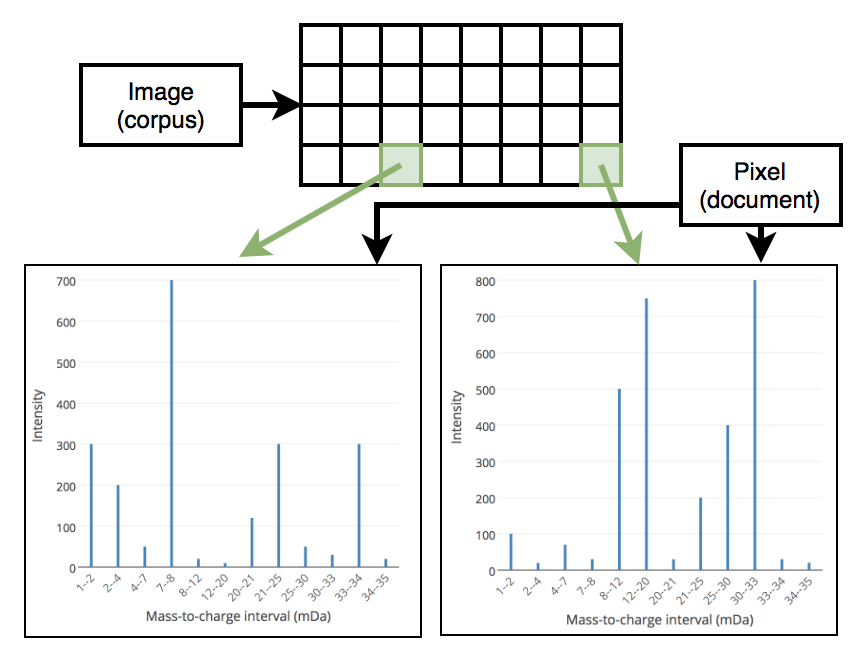
\includegraphics[width=0.42\textwidth]{msi3.png}
  \caption{The MSI data structure.}
  \label{fig:msi}
\end{figure}

% Basis:
% - Unsupervised machine learning: Topic modelling
% - topic modelling w.r.t. MSI
\par Going into the machine learning application, note that we use topic modelling for the inference of topic distributions; effectively, the inferred topic distributions would be treated as the underlying semantic structure of a sampled tissue. Since our data is MSI-based, we model the topic distributions over an image and its every pixel; also, we model the types of ions corresponding to particular topics. Since our machine learning application is based on Bayesian methods, we tune the model parameters to reflect the metabolomics environment as realistically as possible. Ultimately, spatial smoothing is one of such environment settings.

% Research Problem:
% - Noisiness
% -- Fragmentation
% -- Retention time
% - Loss of information
% -- Overlapping topics
\par The basis of the project's research problems comes from the limitations of current metabolite sampling techniques. One of the limitations is the presence of noise. For example, MSI data could be distorted by noise as a result of metabolite fragmentation -- the ionisation would split the metabolite's structure causing a faulty mass-to-charge value capture. Another limitation is the overlap of the molecules with similar structures. Effectively, some of the produced ions could have same mass-to-charge values; as a result, the ion possessing a lower intensity value would be overwhelmed and, thus, not reflected in MSI data. A possible approach mitigating the issue is direct infusion; however, in this project, we investigate whether the latter issue could be mitigated using a computational approach.

% Contributions:
% - A specific and extensive assessment of the SS application
% - A tuned topic model and well-organised experiment settings
\par We contribute to the research in MSI by carrying an extensive assessment of the spatial smoothing application. The assessment is performed in both quantitative and qualitative manners: we assess the performance on a number of diverse datasets; also, our experiments are designed to reflect the environment settings of computational metabolomics. Furthermore, we provide Python implementations of the proposed topic model and the experiment settings. Note that the experiments are performed in Jupyter notebooks; effectively, the practice induces a portable and well-documented environment for initialising and running the experiments. The notebooks are also useful in validating the experiment results: external parties would be able to re-run the experiments in a swift manner.

% The paper's organisation
\par The paper is organised in the following order: in Section 2, we discuss the background of the research project; in Section 3, we provide a formal definition of the assessed research problems; in Section 4, we review the results of the relevant research; in Section 5, we establish the rationale of the applied methodology; in Section 6, we introduce the experiments; finally, in Section 7, we conclude the findings. 

% ___________________________________________________________________________
\section{Background}

% Intro
% - Preliminaries: Introduce the rationale of LDA
% - Terminology: Define the applied topic modelling terminology
% - MSI Data characteristics: Introduce the qualities of the data
\par The background section covers the basis of the concepts used throughout the paper. At the start, we provide a high-level overview of the general topic modelling concepts; then, we define the terminology used throughout the paper; finally, we introduce the characteristic qualities of the MSI data.  
\subsection{Topic Modelling Preliminaries}

% LDA Intro:
% - Hierarchical structure
% - Generative model
% - Bayesian methods
% - Assumptions
\par The research project targets a specific branch of topic models. The branch consists of Latent Dirichlet Allocation (LDA) derivatives. Note that the initial LDA model was introduced by Blei et al. \cite{blei2003latent}. One of the model's key characteristics is the three-level hierarchical treatment of the data. In the context of the utilised MSI data, the hierarchical structure can be perceived as follows: in the highest level, we have an MSI image; in the middle level, we have the pixels of an MSI image; and in the lowest level, we have the intensities of particular ions in a pixel.

% Generatitive model:
% - Generative process
\par Another model's key characteristic is the generative treatment of the data. By a generative model, we mean that the latent data instances are treated as a result of a mixture of underlying parameters. In other words, the generative data treatment induces randomness in the end product of the data generation; however, note that the source of the data -- the lowest level parameters -- remain the same. The key aspect of the generative model is the degree of freedom in the connections of random variables; this notion allows modelling more realistic, thus, more complex data settings. Ultimately, the rationale of a generative machine learning model is based on recovering the underlying semantic structure. To do this, we employ the rationale of Bayesian methods.

% Bayesian methods
% - Inference: sampling
% - Connection to LDA
\par By applying Bayes' rule, we can express the underlying semantic structure in the form of a posterior probability distribution. Since the posterior expression can not always be analytically computed, we estimate it using optimisation or direct sampling. Note that, in this project, we particularly focus on the topic inference using direct sampling. Relating to the attempts for applying the sampling-based inference to LDA-like models, the ground-work was established by Griffiths and Steyvers \cite{griffiths2004finding}. The authors display an application of the collapsed Gibbs sampling -- a Markov chain Monte Carlo (MCMC) algorithm. Since the method integrates the uncertainty out, we can sample the data entities without the explicit notion of the underlying parameters.

% Assumptions
% - Exchengeability (BoW)
% - Discrete data
\par Going back to the initial LDA model, the model's authors report on setting the following assumptions: exchangeability among the inner components of the lower and middle data hierarchy levels; and a discrete treatment of the lower-level data. By exchangeability, it is meant that the components follow the bag-of-words principle; that is, the order of the data has no correlation with the underlying semantic structure. Relating to the rationale behind the discrete data treatment, it is assumed that the lower-level components have no spatial connection. With respect to our project, both assumptions -- the exchangeability and the discreteness -- do not correspond to the characteristics of the metabolomics environment. Therefore, we establish a methodology to relaxing the latter assumptions.

\subsection{Topic Modelling Terminology}

% Terminology intro:
% - Introduce the three-level hierarchical structure
\par In this subsection, we introduce our topic modelling terminology. In order to put the MSI data structure in the topic modelling context, the components of LDA's three-level hierarchical structure are defined as follows: \textit{a corpus} is the whole image of a sample; \textit{a document} is an MSI image's pixel; and \textit{a word} is an interval of mass-to-charge values corresponding to a particular ion. Note that from now on, we use the latter topic modelling concepts to introduce the LDA model's architecture and notation.

% LDA design
% - Graphical model
\par Since LDA-like models correspond to the branch of graphical models, the dependence of random variables can be illustrated using graphs. In order to familiarise with the architecture and the variables of LDA-like models, we provide Figure \ref{fig:arch_LDA-init} illustrating the initial LDA model in the plate notation.
\begin{figure}[h]
  \centering
  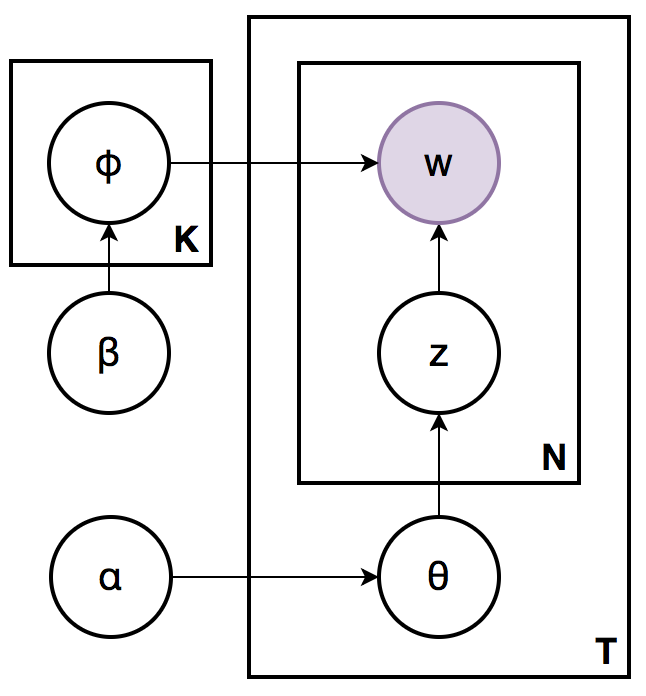
\includegraphics[width=0.20\textwidth]{LDA-initial.png}
  \caption{The initial LDA model's architecture.}
  \label{fig:arch_LDA-init}
\end{figure}
To start with, the circles indicate the model's variables: the coloured circle corresponds to the observable variable; and the uncoloured circles correspond to the hidden variables. Effectively, the hidden variables define the model's underlying structure. To introduce the plates, the plate denoted by $K$ corresponds to the number of topics; the plate denoted by $T$ corresponds to the number of documents, and the plate denoted by $N$ corresponds to the number of words. Effectively, the letters in the bottom right corners indicate the total number of variables. Therefore, a corpus has a $T$ number of documents, and each document has an $N$ number of words.

% Terminology
% - Parameter meaning
% - Listing
\par Before providing a listing with the definitions of the LDA variables, we introduce their purpose. The variables denoted by $\theta$ and $\phi$ correspond to the underlying probability distributions (e.g., in the case of the initial LDA model, we use Dirichlet distributions). It follows that the variables denoted by $\alpha$ and $\beta$ act as the parameters of the latter probability distributions; note that in the context of machine learning, such auxiliary parameters are called hyper-parameters. Effectively, \textit{a hyper-parameter} allows tuning a machine learning model for a particular dataset application. As a side reference, note that by \textit{a vocabulary} we refer to a collection of terms reflecting a fixed range of words. At this point, we provide the following list containing the definitions of the initial LDA model's variables: 
\begin{itemize}
	\item $K$ is the number of topics;
	\item $T$ is the number of documents;
	\item $N$ is the number of words per document;
	\item $V$ is the size of a vocabulary;
	\item $w$ is a word;
	\item $z$ is a word's topic assignment;
	\item $\theta_t$ is the topic distribution over the document $t$;
	\item $\phi_k$ is the vocabulary term distribution over the topic $k$;
	\item $\alpha$ is the hyper-parameter for the topic distributions;
	\item $\beta$ is the hyper-parameter for the vocabulary term distributions.
\end{itemize}

\subsection{MSI Data Characteristics}

% MSI dataset intro:
% - Introduce the raw data format
% - Describe the data pre-processing requirements
\par In this subsection, we introduce the qualities of the MSI data. Furthermore, we set the requirements for the pre-processing of raw MSI data; note that the pre-processing serves as an auxiliary method making raw MSI data compatible for a scalable topic modelling application. As a side note, the basis of our applied MSI data characteristics is established from the mzML data format. Conveniently, we parse mzML data using the \texttt{pymzml} Python library. 

% Raw data format
% - Data meaning
% - Explain the raw data by looking into it
\par Recall that raw MSI data is mass spectra of a tissue's sample (i.e., the sample's every pixel is expressed in the form of a mass spectrum); also, every mass spectrum term conveys a particular intensity value. To help organise the data, we establish a continuous notion by ordering the mass-to-charge values. Further, since the sampling equipment can detect the mass-to-charge values in the millidalton (\textit{mDa}) precision, the MSI data is sparse (i.e., a large portion of mass-to-charge values are mapped to the zero intensity). 

% Data pre-processing requirements
% - Vocabulary generation
% - Intensity normalisation
% - Dismissing inferior information
\par In the context of topic modelling, raw MSI data possess a large vocabulary (above $5000$ terms). Note that we consider every mass-to-charge value as a word; whereas every intensity value is perceived as a word's occurrence count. Further, since the intensity values could spike up above $1000$, the time complexity of the latent topic inference would require pro-longed runs. To overcome the introduced scalability issues, we carry data pre-processing (the applied techniques are discussed in the upcoming methodology section).

% ___________________________________________________________________________
\section{Statement of Problem}

% Hypothesis
% - A topic is continuous throughout nearby regions
\par To start with, we set the hypothesis of this research project to \textit{`The spatial smoothing application induces more realistic representation of the visual computational metabolomics data -- MSI'.} By spatial smoothing, it is meant that the topic model would have an auto-regressive treatment among the nearby MSI instances. As an example, we assume that adjacent pixels would have similar latent topic distributions. This assumption corresponds to the nature of our datasets -- a metabolite construction (i.e., a topic) is continuous throughout nearby regions (i.e., sets of adjacent pixels).

% Contributions
% - Naive AR model application
% - Motivating for the state-of-the-art AR model application
\par The impact of proving the hypothesis would bring the following contributions:
\begin{itemize}
	\item Improve the detection of overlapping topics and vocabulary terms;
	\item Reduce the noisiness of the MSI data;
	\item Motivate a further research in the spatial smoothing application in MSI data.
\end{itemize} 
To expand on the overlapping topic detection, the issue arises when two underlying topics are made of similar vocabulary terms: instead of a separate representation, the topics are merged. We intend to identify the flow of distinct topics by applying spatial smoothing; as a consequence, the spatial smoothing would also impact the data noisiness reduction. Ultimately, if a naive spatial smoothing application displayed a performance improvement, the contribution would set a basis to utilise state-of-the-art auto-regression techniques in MSI data.

% Approach
% - Clearly define the experiment settings
% - Tune the models by studying synthetic datasets.
\par To my knowledge, the impact of applying spatial smoothing to MSI data has not yet been thoroughly studied. For the latter reason, this research project serves as an exploratory assessment -- we introduce the rationale behind the applied methodology; also, we clearly define the range of the experiment settings. To give a brief intuition about the methodology, the study assesses the domain-specific parameter tuning and its impact on a range of synthetic datasets.

% ___________________________________________________________________________
\section{Relevant Research}

% Intro (separate into three)
% - MSI DATA:
% -- alonso2015analytical
% -- Review the metabolomics feature pre-processing
% -- Review the metabolomics alternative approaches
% - Review the implementation approaches
% -- blei2012probabilistic
% -- Gibbs sampling
% -- DTM
\par In this section, we review the ground-work carried on the following aspects: the pre-processing of MSI data; the rationale of the utilised topic models; and novel approaches exploiting the characteristics of MSI data. Note that the covered groundwork is selected to reflect the rationale of the utilised techniques. In order to establish the basis of the state-of-the-art computational metabolomics methodology, we consult the survey carried by Alonso et al. \cite{alonso2015analytical}; to introduce the key probabilistic topic modelling branches, we consult the survey carried by Blei \cite{blei2012probabilistic}. 

\subsection{MSI Data Pre-processing}

% Metabolomics: feature pre-processing
% - Normalisation:
% -- kohl2012state
% -- bolstad2003comparison

\par In order to establish a scalable topic inference, we review the following MSI data pre-processing techniques: data normalisation; feature binning; and noise reduction. To start with, data normalisation serves as a method establishing an adaptable data structure. Bolstad et al. \cite{bolstad2003comparison} have proposed the data normalisation method called linear baseline scaling. Note that the method is particularly targeted at sparse datasets. Effectively, the method is applicable to numerical features; note that the method's work-flow is carried as follows: we find the largest numerical feature of all data instances; then, we calculate the scaling factors by aligning the largest values to a pre-set upper threshold; finally, we align the remaining numerical features based on the established scaling factors. Relating linear baseline scaling to applications on MSI data, Kohl et al. \cite{kohl2012state} have shown that the method's application does not produce a significant loss of information to establish a well-performing MSI data inference. 

% - Binning
% -- Evenly spaced 
% -- craig2006scaling
% -- Spectral peaks
% -- de2008nmr
\par To introduce feature binning, the technique is used to merge the instances of a feature space; as a result, feature binning reduces the data dimensionality. Note that by the MSI data feature space, we refer to distinct $m/z$ values. Since raw MSI data is sparse, a successful application of feature binning is based on identifying appropriate $m/z$ boundaries reflecting unique metabolite types. To introduce some examples, the research carried by Craig et al. \cite{craig2006scaling} have utilised an equally spaced feature binning. Even though the authors have succeeded to reduce the data dimensionality, they have encountered a loss of information by splitting the metabolite topics into arbitrary regions. As an alternative approach, De et al. \cite{de2008nmr} have performed a feature binning based on the identification of spectral peaks. Effectively, the technique induces a dynamic notion of bin boundaries which are based on the identified intensity peak regions. As a result, the merged $m/z$ values serve as a better representation of metabolite terms.

% - Denoising (removing small intensities)
% -- smith2014proteomics
\par The last reviewed MSI data pre-processing techniques addresses the MSI data noisiness. Even though the MSI data noise reduction is an open research problem utilising techniques beyond data pre-processing, Smith et al. \cite{smith2014proteomics} have shown that the application of a general data pre-processing routine displays performance improvements. For example, the authors have induced a lower intensity bound. Effectively, the intensity values below the intensity threshold would be treated as insignificant and/or as a product of data capturing device imperfections. By applying this procedure, the authors have successfully reduced the data dimensionality and, thus, increased the data scalability.

\subsection{Prospective Topic Models}

% Intro
% - Inference
% - Derivatives
% - Gibbs sampling
% -- griffiths2004finding
\par In this subsection, we review the key characteristics of the prospective topic modelling inference techniques and model variations. To apply the inference techniques, we employ the rationale of a sampling-based LDA model. Griffiths and Steyvers \cite{griffiths2004finding} have displayed a successful application of the collapsed Gibbs sampler for the topic inference of both textual and visual data. To expand on the collapsed sampling, the technique allows skipping the estimation of the $\theta$ and $\phi$ values; instead, the inference is based on the notion of the assignment counts. In order to estimate a topic assignment's probability, the authors suggest using the following expression:
\begin{equation*}
P(z_i = k | z_{-i}, w) \propto \dfrac{n_{-i, k}^{(w_i)} + \beta}{n_{-i, k}^{(\cdot)} + V\beta}\cdot \dfrac{n_{-i, k}^{(t_i)} + \alpha}{n_{-i, \cdot}^{(t_i)} + K\alpha}.
\end{equation*}
Note that $i$ refers to the current iteration ($-i$ refers to the previous iteration); $k$ refers to a particular topic; and $n$ refers to the count of the instances indicated by the term's superscript. If required, $\theta$ and $\phi$ can be sampled from the following distributions:
\begin{align*}
\phi_{k,w} & \sim \mbox{Dirichlet}\bigg(\dfrac{n_{k}^{(w)} + \beta}{n_{k}^{(\cdot)} + W\beta}\bigg),\\
\theta_{t,k} & \sim \mbox{Dirichlet}\bigg(\dfrac{n_{k}^{(t)} + \alpha}{n^{(t)} + K\alpha}\bigg).
\end{align*}
Essentially, more accurate representations of $\theta$ and $\phi$ are obtained by running the Gibbs sampler until a sufficient convergence: we preserve the $\theta$ and $\phi$ values of each iteration; when the sampling is finished, the average of the preserved values is an accurate approximation of the underlying $\theta$ and $\phi$ values.

% Topic modelling:
% - DTM
% -- blei2006dynamic
% - SeqLDA
% -- du2012sequential
\par In order to relax the topic modelling assumptions of the initial LDA model, we review the model's derivatives. One of the assumptions -- word exchangeability -- is addressed by Blei and Lafferty \cite{blei2006dynamic}. 
The authors have proposed dynamic topic model (DTM) inducing the notion of change in the topic and vocabulary distributions; the model's architecture is illustrated in Figure \ref{fig:arch_dtm}.
\begin{figure}[h]
  \centering
  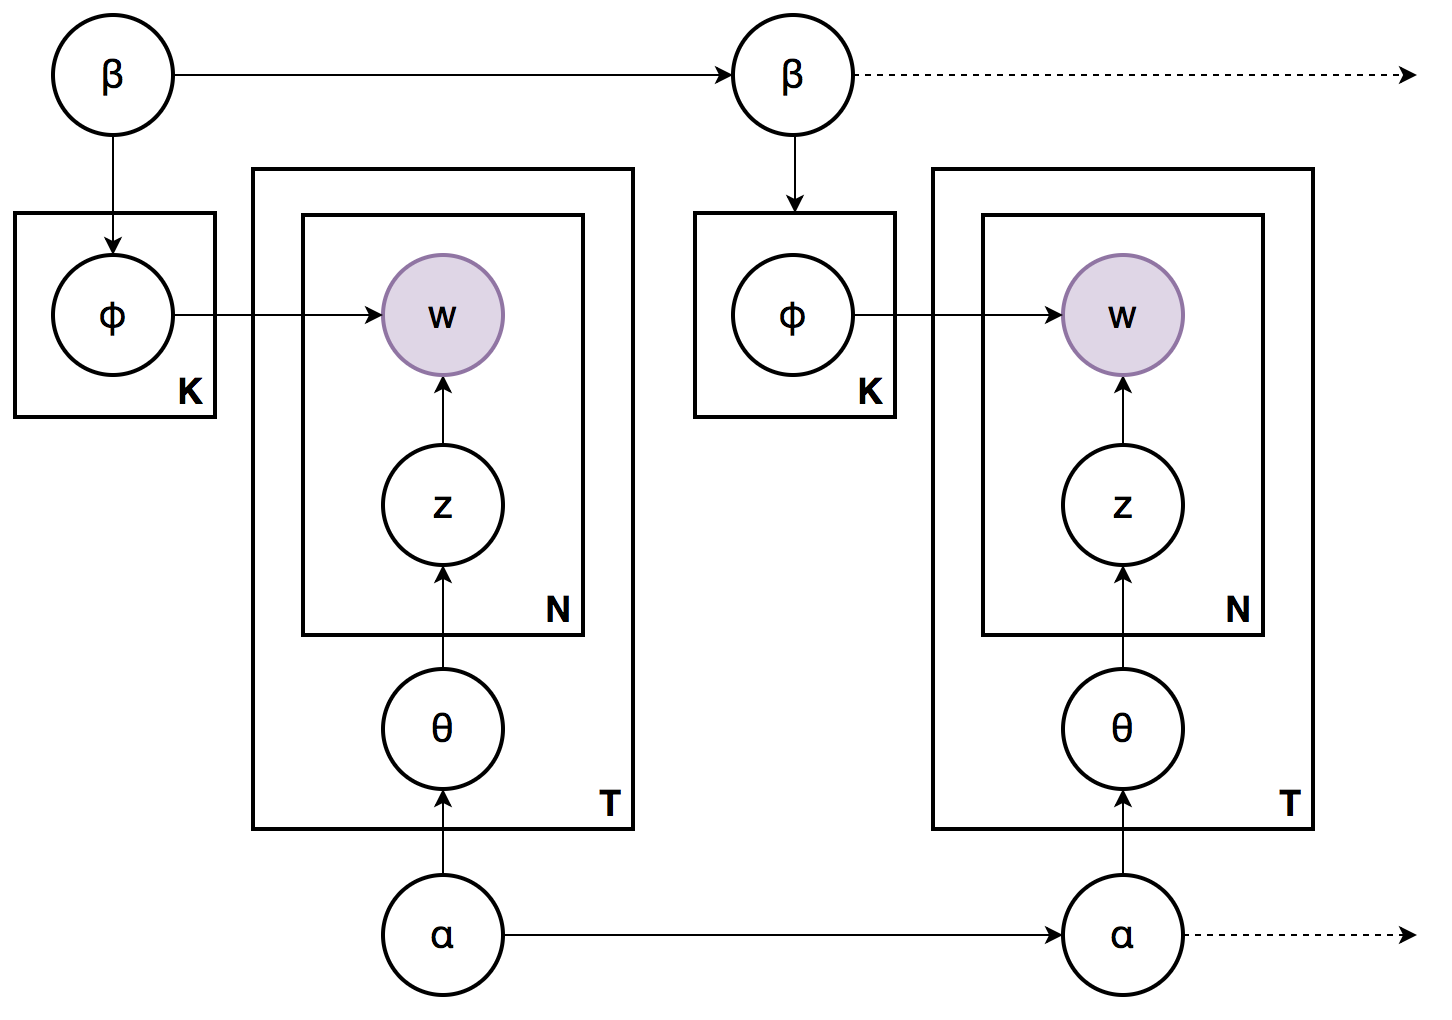
\includegraphics[width=0.4\textwidth]{dtm-architecture.png}
  \caption{The DTM architecture.}
  \label{fig:arch_dtm}
\end{figure}
Ultimately, the documents of a corpus are assigned to segments with unique $\theta$ and $\phi$ values. Note that the changes in the $\theta$ and $\phi$ values are impacted by their hyper-parameter updates. Since, in the DTM paper, the authors use variational inference, we provide a reference for an alternative dynamic topic modelling variation -- sequential LDA -- proposed by Du et al. \cite{du2012sequential}. Note that in the sequential LDA paper, the authors display a rigorous application of the collapsed Gibbs sampler. 

\subsection{Prospective Characteristics of MSI Data}
% Metabolomics: spatial smoothing
% - TM application
% -- van2016topic
\par At this point, we look into the prospective topic modelling applications exploiting the characteristics of MSI data and employing spatial smoothing. To start with, Hooft et al. \cite{van2016topic} have utilised an LDA-like model to infer metabolite substructures from MSI data. The authors have established a novel approach utilising a favourable LDA's property -- the option to assign a unique vocabulary term to multiple topics. Effectively, this approach allows identifying metabolite substructures which are made of overlapping elements. 

% - Spatial Chaos
% -- palmer2016fdr
\par Relating to the spatial smoothing application, to my knowledge, the idea has not yet been widely spread among the computational metabolomics community. Nevertheless, a recent study by Palmer et al. \cite{palmer2016fdr} have attempted to quantify spatial chaos among the partitions of MSI data. The authors have reported that the established notion of spatial chaos has improved the speed and accuracy of continuous metabolite pattern identification. 


% ___________________________________________________________________________
\section{Methodology}

% Intro
\par In this section, we cover the rationale of the topic model tuned for the spatial smoothing application. To start with, we provide details on how to establish the auto-regressive notion among MSI data; then, we show how to apply the auto-regression to the topic inference based on the collapsed Gibbs sampling. Further, we provide a list of the applied data pre-processing techniques for MSI data. Finally, considering the data format induced by data pre-preprocessing, we introduce the generative MSI data process. Effectively, we apply the generative process to generate synthetic data for our experiments.

\subsection{Spatial Smoothing}

% Introduce AR
% - Define the first two variances
% - Point out that we are using the terms corresponding to the MSI data
\par We establish the spatial smoothing among MSI data by inducing the auto-regressiveness among pixels (documents). Before going into details, note that we cover the established methods using the previously introduced topic modelling notation. To start with, recall that by auto-regressiveness we refer to the smooth topic development among the nearby instances of an MSI corpus. In our settings, the auto-regressiveness is established by assuming that the joint probability distribution of the $\alpha$ priors is given by the following expression:
\begin{align*}
&p(\alpha_1,\ldots,\alpha_T) =p(\alpha_1)\prod_{t=2}^{T}{p(\alpha_t|\alpha_{t-1})}, \quad \mbox{where}\\
&p(\alpha_0) =\mathcal{N} (\alpha_0; 0, \sigma_0^2I), \quad \mbox{and}\\
&p(\alpha_t) =\mathcal{N} (\alpha_t; \alpha_{t-1}, \sigma^2I), \quad t>0.
\end{align*}
To introduce the previous expression, note that the index $t$ refers to a particular pixel (a document). This means that every pixel of an MSI corpus has a unique underlying topic distribution induced by a unique $\alpha$. Further, the variances $\sigma_0^2$ and $\sigma^2$ correspond to the initialisation variance and the smoothness variance, respectively. Effectively, $\sigma_0^2$ is used to create larger gaps among different topics, whereas $\sigma^2$ preserves the smoothness. Therefore, we set $\sigma_0^2$ to possess a higher value compared to $\sigma^2$.

% Introduce the MH algorithm
\par The previously introduced $\alpha$ priors serve as the initial point in estimating the true $\alpha$ values. To estimate the true $\alpha$ values, we utilise the Metropolis--Hastings (MH) algorithm. The work-flow of the MH algorithm is started by drawing the proposed state:
\begin{align*}
&x' \sim q(x,\delta^2I).
\end{align*}
Note that $x$ denotes the current state, $q$ denotes the proposal distribution, and $\delta^2$ denotes the proposal variance; also, note that if $\delta^2$ is large, the proposal state converges to the true posterior in larger yet random increments; alternatively, if $\delta^2$ is small, the convergence is performed in small yet uniform increments. Note that the settings for an optimal convergence are unique for diverse datasets; as an example, we can find the optimal values using cross validation. Going back to the work-flow, for the second step, we consider the acceptance distributions (these are denoted by $A$) and derive the formula for the acceptance rate:
\begin{align*}
  \dfrac{A(x'|x)}{A(x|x')} = \dfrac{p(x'|x)}{p(x|x')}\cdot \dfrac{q(x'|x)}{q(x|x')} = \dfrac{p(x',x)}{p(x)}\cdot \dfrac{p(x')}{p(x,x')} = \dfrac{p(x')}{p(x)}.
\end{align*}
Note that the proposal distributions cancel out as
\begin{align*}
q = \mathcal{N} \quad \Longrightarrow \quad q(x'|x) = q(x|x').
\end{align*}
For the MH algorithm's final step, we make sure that the acceptance rate does not overflow the probability boundaries; that is, we obtain the acceptance rate denoted by $r$ using the following procedure:
\begin{align*}
  r = \min{\bigg(1, \dfrac{p(x')}{p(x)}\bigg)}.
\end{align*}

% Apply the MH algorithm to the MSI data
% TODO: Softmax
\par At this point, we apply the rationale of the introduced MH algorithm to the topic modelling context. Since we utilise the MH algorithm to update a single value at a time (i.e., we update $\alpha_{t,k}$), we make use of the following notation:
\begin{align*}
  \alpha^{-tk} = \alpha \setminus \alpha_{t,k}.
\end{align*} 
Having the previous notation in mind, the MH algorithm's application to update $\alpha$ is given as follows:
\begin{align*}
  &\dfrac{p(z,\alpha^{-tk},\alpha_{t, k}'|X)}{p(z,\alpha|X)} = \ldots\\
  &\ldots = \dfrac{p(X|z,\alpha^{-tk},\alpha_{t, k}')}{p(X|z,\alpha)}\cdot \dfrac{p(z|\alpha^{-tk},\alpha_{t, k}')}{p(z|\alpha)}\cdot \dfrac{p(\alpha^{-tk},\alpha_{t, k}')}{p(\alpha)}\\
  &\dots = \dfrac{\prod_{k=1}^K\pi(\alpha_{t,k}')^{z_{t,k}}\cdot p(\alpha_t'|\alpha_{t-1})\cdot p(\alpha_{t+1}|\alpha_t')}{\prod_{k=1}^K\pi(\alpha_{t,k})^{z_{t,k}}\cdot p(\alpha_t|\alpha_{t-1})\cdot p(\alpha_{t+1}|\alpha_t)};\quad t \not\in \{1,T\}.
\end{align*}
For completeness, the expressions at the boundaries take the following form:
\begin{align*}
t=1 \quad \Longrightarrow \quad &\dfrac{p(\alpha^{-1k},\alpha_{1, k}')}{p(\alpha)} = \dfrac{p(\alpha_{1}')\cdot p(\alpha_{2}|\alpha_{1}')}{p(\alpha_{1})\cdot p(\alpha_{2}|\alpha_{1})},\\
t=T \quad \Longrightarrow \quad &\dfrac{p(\alpha^{-Tk},\alpha_{T, k}')}{p(\alpha)} = \dfrac{p(\alpha_{T}'|\alpha_{T-1})}{p(\alpha_{T}|\alpha_{T-1})}.\\
\end{align*}
Also, note that by $\pi$ we denote the softmax function which is expressed as follows:
\begin{align*}
  \pi(\alpha_{t,k}) = \dfrac{\exp(\alpha_{t,k})}{\sum_{k'=1}^K \exp(\alpha_{t,k'})}
\end{align*} 

\subsection{Auto-regressive Dynamic Topic Model}

% Intro
% - Model modifications
\par Our auto-regressive topic model is based on the rationale of the reviewed dynamic topic model. However, based on the MSI data characteristics and the application of spatial smoothing, the auto-regressive model possesses the following aspects:
\begin{itemize}
	\item The static treatment of the $\beta$ hyper-parameter;
	\item The Gibbs sampler utilising spatial smoothing;
	\item The application of logarithmic space to perform calculations.
\end{itemize}
In the following paragraphs, we introduce each of the previous listings.

\par Even though we utilise the rationale of DTM in order to establish the dynamic notion of the topic development, we preserve a static $\beta$ hyper-parameter. This assumption comes from the characteristics of the metabolomics-based MSI data: we expect the metabolite patterns (i.e., a topic's vocabulary) remain constant. Therefore, in our model, we utilise the architecture illustrated in Figure \ref{fig:arch_ar} below.
\begin{figure}[H]
  \centering
  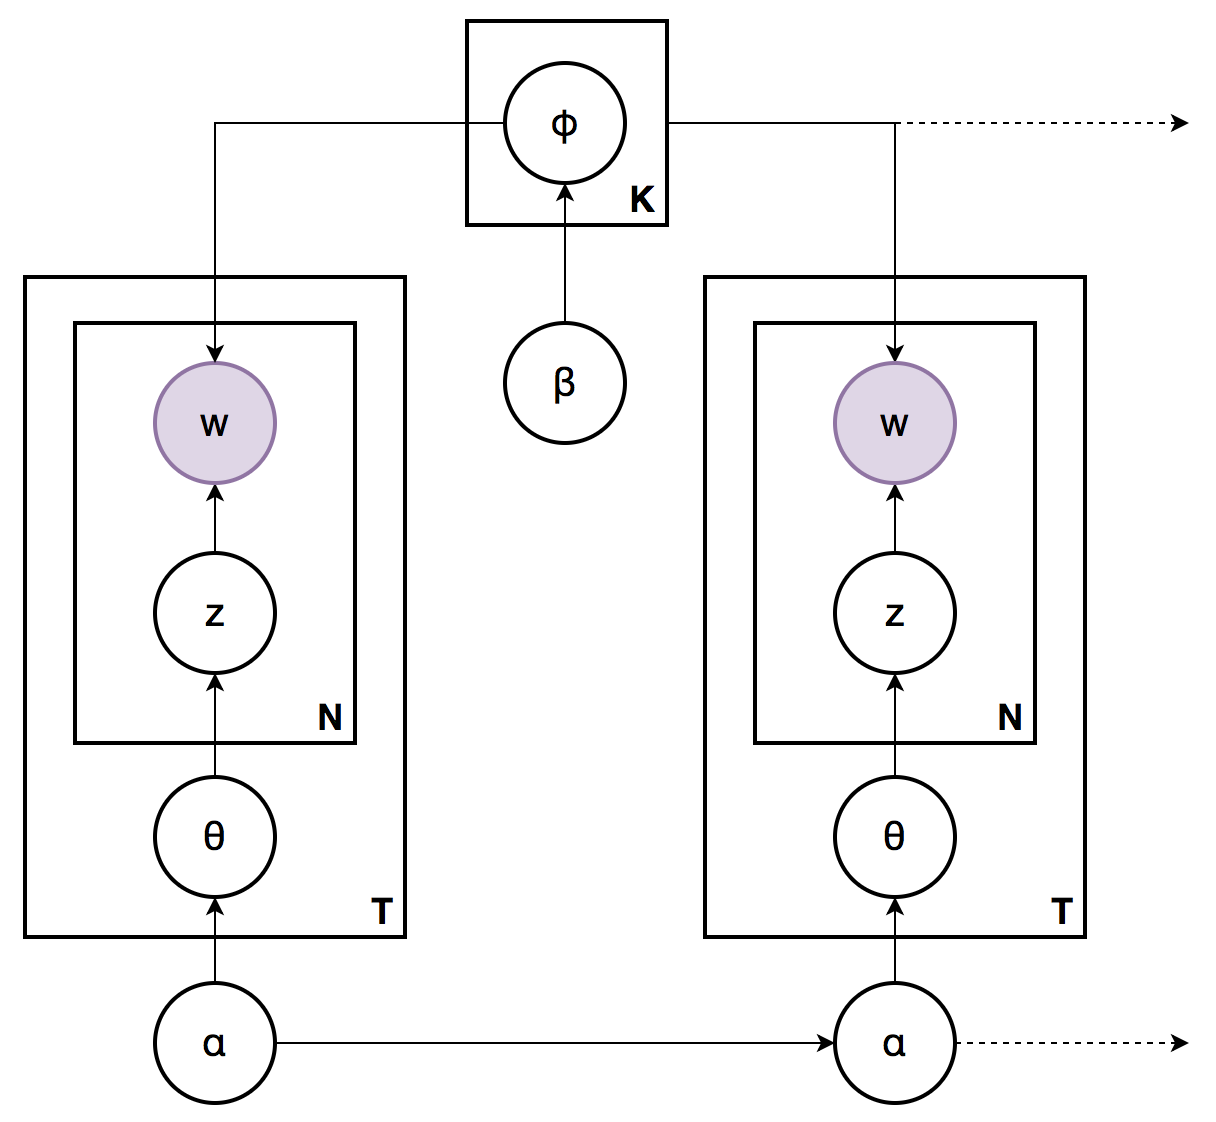
\includegraphics[width=0.33\textwidth]{ar-architecture.png}
  \caption{The auto-regressive topic model architecture.}
  \label{fig:arch_ar}
\end{figure}

% Gibbs Sampler changes
\par In order to enhance the Gibbs sampler, we modify the topic assignment formula to take the following form:
\begin{equation*}
P(z_i = k | z_{-i}, w, t) \propto \dfrac{n_{-i, k}^{(w_i)} + \beta}{n_{-i, k}^{(\cdot)} + V\beta}\cdot \pi(\alpha_{t,k}).
\end{equation*}
As a consequence, the sampling of $\theta$ also changes; now, we obtain the topic distribution as follows:
\begin{align*}
\theta_{t,k} = \pi(\alpha_{t,k}).
\end{align*}

% Calculations in the log space
\par Finally, we address the computational stability by performing calculations in logarithmic space. Effectively, the application of logarithmic space mitigates the susceptibility to numerical underflow. Note that numerical underflow is especially relevant in the context of probabilistic models: calculations involve large products of probabilities. In logarithmic space, however, the products are transformed into sums. Relating to our model, we apply logarithmic space for both the auto-regressive $\alpha$ update and the sampling-based inference. The updated expression for the auto-regressive $\alpha$ update is given as follows:
\begin{alignat*}{2}
  &\log&&\bigg[{\dfrac{p(z,\alpha^{-tk},\alpha_{t, k}'|X)}{p(z,\alpha|X)}}\bigg] = \ldots \\
  & \ldots && = \log\big[{p(z,\alpha^{-tk},\alpha_{t, k}'|X)}\big] - \log\big[{p(z,\alpha|X)}\big]\\
  & \ldots && = z_{t}\sum_{k=1}^K\log\big[\pi(\alpha_{t,k}')\big] + \log\big[p(\alpha_t'|\alpha_{t-1})\big] + \log\big[p(\alpha_{t+1}|\alpha_t')\big]\\
  & && - z_{t}\sum_{k=1}^K\log\big[\pi(\alpha_{t, k})\big] + \log\big[p(\alpha_t|\alpha_{t-1})\big] + \log\big[p(\alpha_{t+1}|\alpha_t)\big].
\end{alignat*}
As a result, the acceptance rate takes the following expression:
\begin{align*}
	r_{t,k} = \exp\big[\min{\big(0, \log\big[{p(z,\alpha^{-tk},\alpha_{t, k}'|X)}\big] - \log\big[{p(z,\alpha|X)}\big]}\big)\big].
\end{align*}
To introduce the updated expression for the inference, it is expressed as follows:
\begin{align*}
&P(z_i = k | z_{-i}, w, t) \propto \ldots\\
&\ldots \propto \log\big[n_{-i, k}^{(w_i)} + \beta\big] - \log\big[n_{-i, k}^{(\cdot)} + V\beta\big] + \log\big[\pi(\alpha_{t,k})\big].
\end{align*}

\subsection{Data Pre-processing and Generative Process}

% Intro
% - The purpose of the real data
% - Introducing the applied generative process
\par In this subsection, we introduce the MSI data format used in the experiments. At the start, we introduce an example of real data. Effectively, the example displays an application of the pre-processing techniques presented in the literature review section. Further, we transfer the qualities of real MSI data into our synthetic data generation module. To be more specific, we provide an algorithm for the generative data process.

% Looking into real data
% - Applying the reviewed pre-processing techniques
% -- low intensity
% -- bucketisation

\par Before carrying the experiments, we familiarise with raw MSI data characteristics and assess their scalability. To be more specific, we define the characteristics of our synthetic data by pre-processing a real MSI data sample. To introduce the pre-processing details, we dismiss the words below the intensity threshold of $10$; then, we apply the following bucketisation strategy: merge adjacent vocabulary terms which differ less than $7$ \textit{mDa}. Effectively, the bucketisation strategy is based on the spectral peak identification. Finally, we apply linear baseline scaling to align the highest intensities to $25$. Most importantly, note that these settings are unique with every dataset; however, the provided values allow carrying experiments in a scalable manner (i.e., a single experiment run on one dataset would take approximately $60$ minutes).

% Plots of pre- and past-normalisation
% - Preserving the metabolotite patterns
% - Improving the scalability (inference iteration time)
\par At this point, we take an exemplary sample. Note that, in the sample, there are two letters inscribed with the ink corresponding to a particular mass-to-charge value. In Figure \ref{fig:comparison}, we compare the visualisation of the sample with and without the applied pre-processing.

\begin{figure}[H]
  \centering

  \begin{subfigure}[b]{0.5\textwidth}
    \caption{The `b and e' term's occurrences before linear baseline scaling.}
    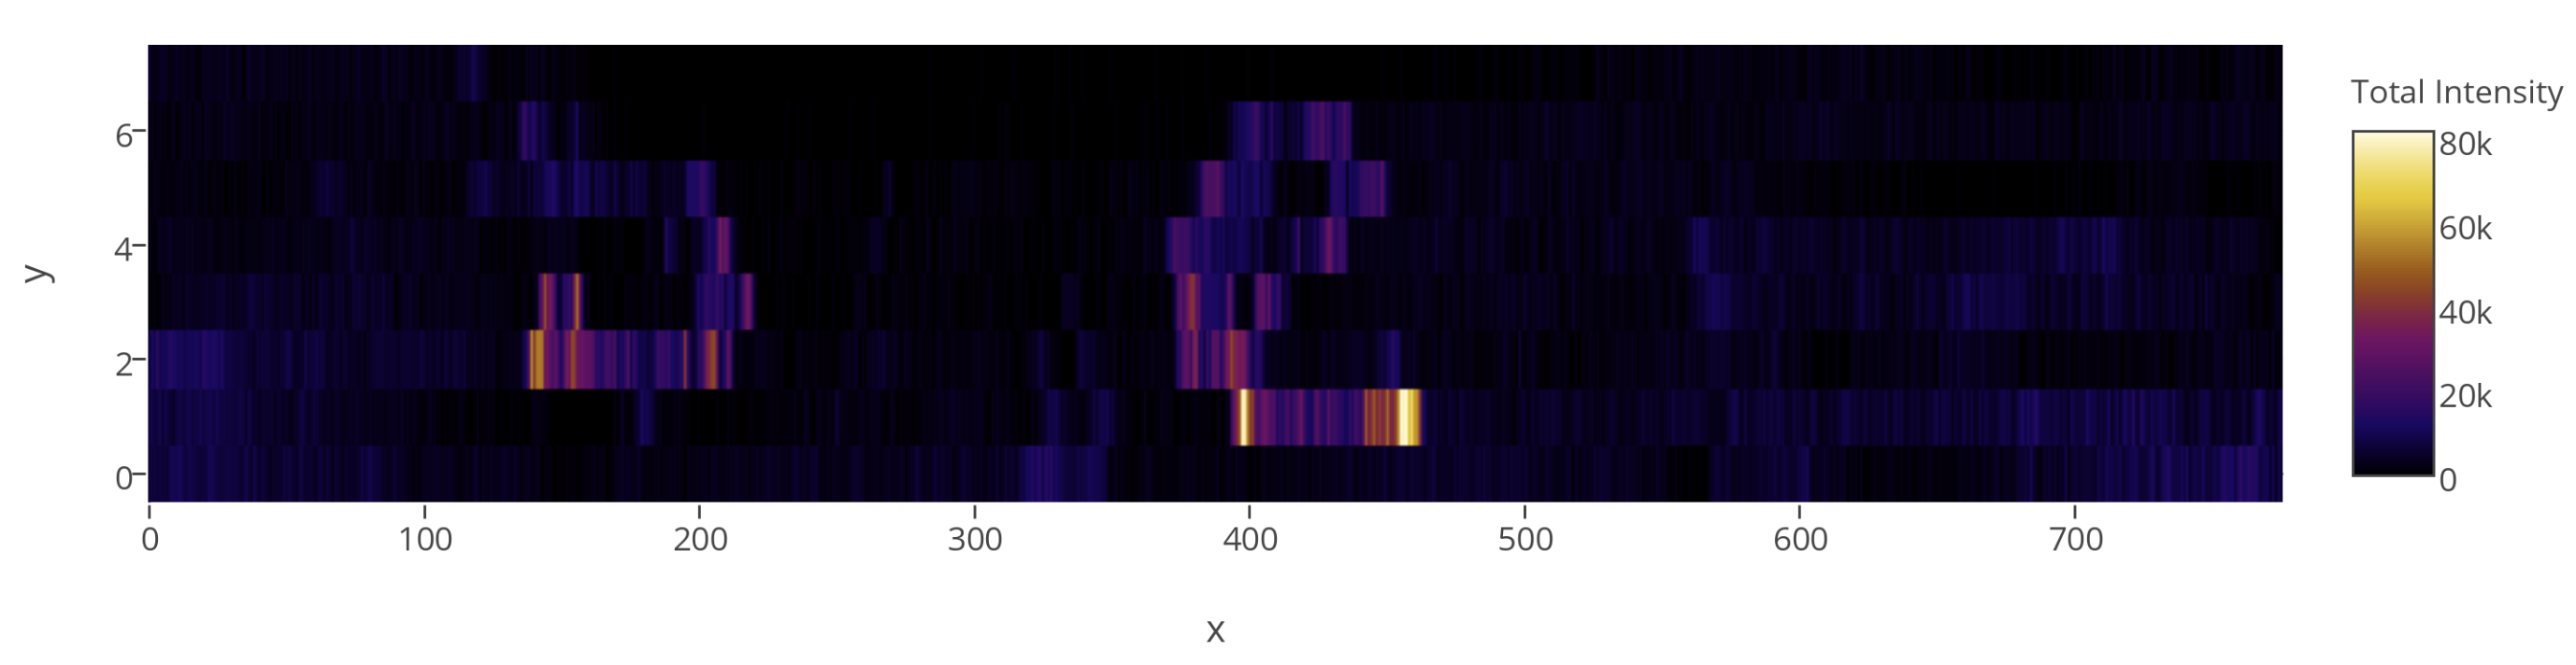
\includegraphics[width=\linewidth]{pre.png}
  \end{subfigure}%

  \begin{subfigure}[b]{0.5\textwidth}
    \caption{The `b and e' term's occurrences after linear baseline scaling.}
    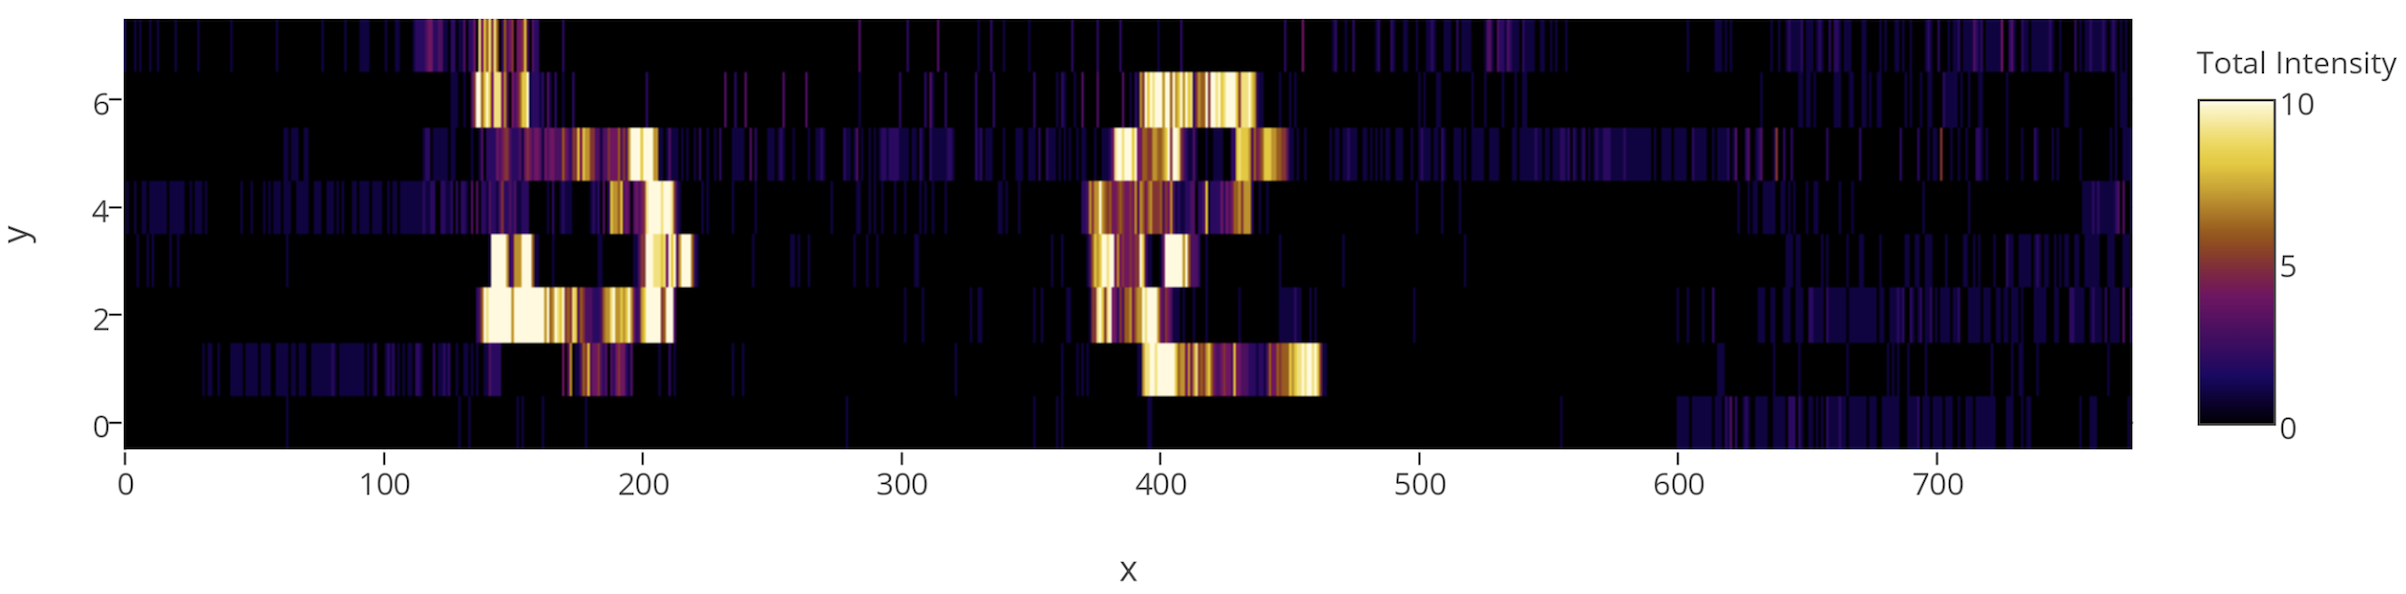
\includegraphics[width=\linewidth]{post.png}
  \end{subfigure}%

  \begin{subfigure}[b]{0.5\textwidth}
    \caption{An inferred topic corresponding to the `b and e' pattern.}
    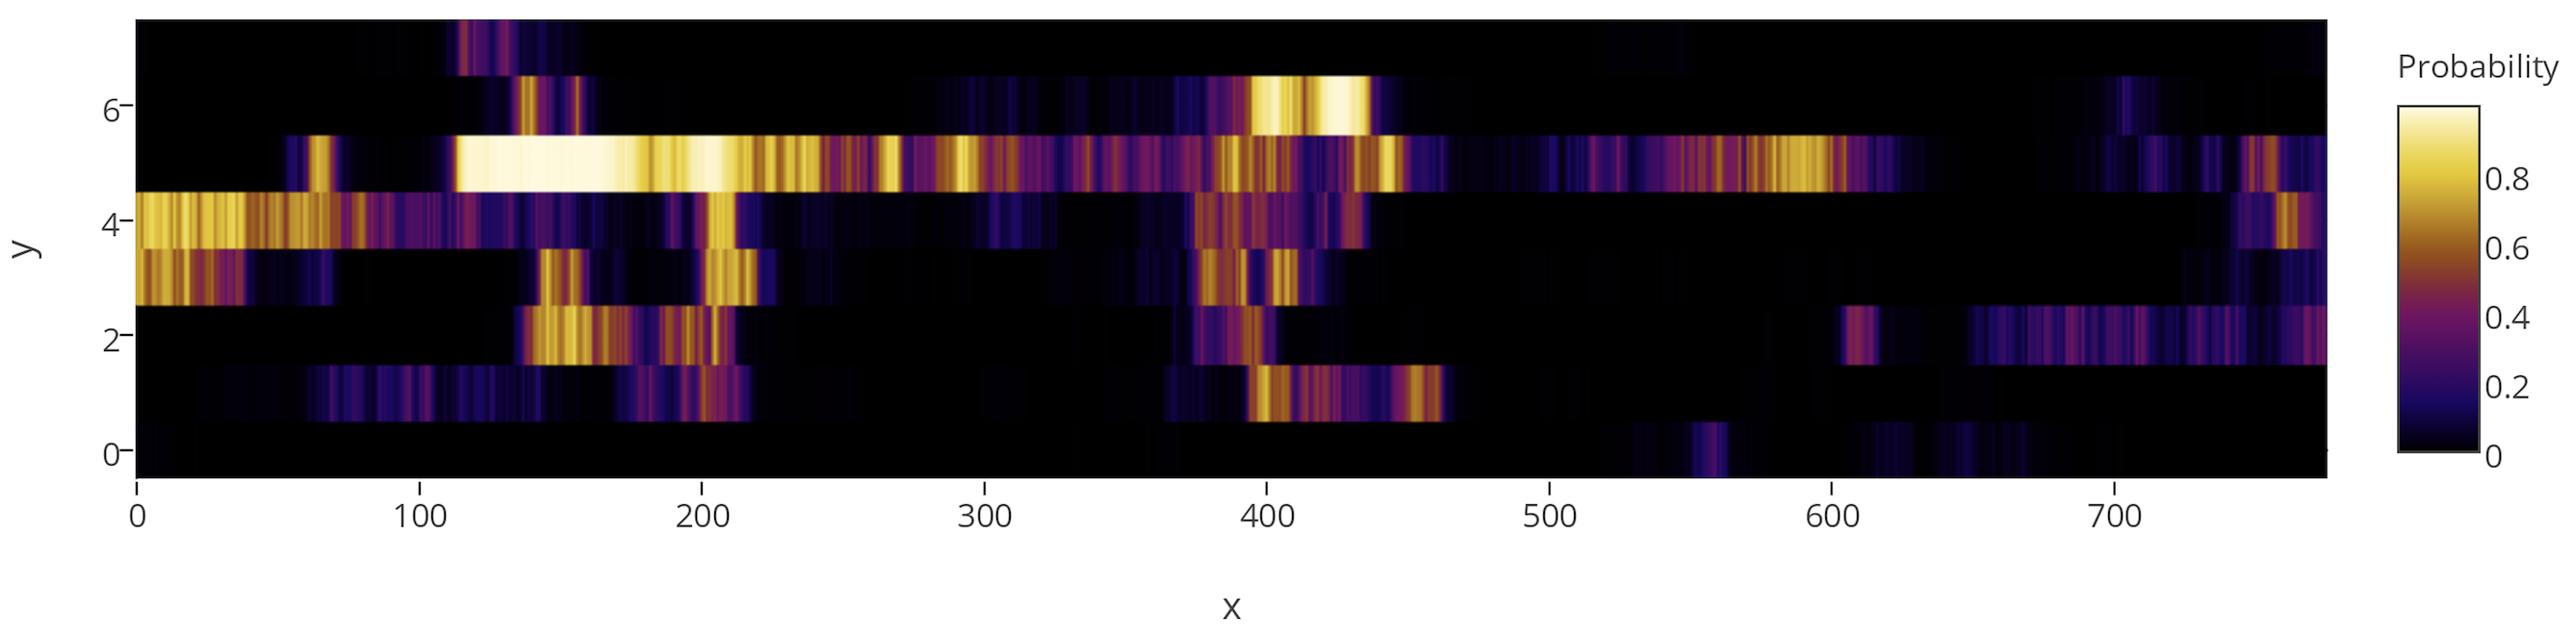
\includegraphics[width=\linewidth]{topic.png}
  \end{subfigure}%
  \caption{The comparison of the `b and e' term's extraction.}
  \label{fig:comparison}
\end{figure}

% The generative process
% - The underlying assumption for the inference
% - synthetic data
% -- Large amounts of data
% - The algorithm of the generative process
% - 1 document is 1 segment
\par Having the basis for a scalable inference, we transfer the identified data properties into the synthetic corpus generation. Before introducing the generative process, recall that our dynamic topic treatment is unique with respect to every document. Therefore, contrary to the reviewed dynamic topic models, our dynamic segment consists of only one document. Considering the latter aspects, we establish our utilised generative using Algorithm \ref{alg:dynamic_document_generation} given below:
\begin{algorithm}[H]
\caption{The generative process for a synthetic corpus.}
\label{alg:dynamic_document_generation}
\begin{algorithmic}[2]
% \State $\alpha_0 \sim \mathcal{N}(0, \sigma_0^2I)$
\For {$t \leftarrow 1, T$}
% \State $\alpha_t \sim \mathcal{N}(\alpha_{t-1}, \sigma^2I)$
\State $N \sim \mbox{Poisson}(\xi)$
\For {$n \leftarrow 1, N$}
\State $z_{t, n} \sim \mbox{Multinomial}(\pi(\alpha_t))$
\State $k = \{i : z_{t, n, i} = 1\}$
\State $w_{t, n} \sim \mbox{Multinomial}(\phi_k)$
\EndFor
\EndFor
\end{algorithmic}
\end{algorithm}
In practical settings, the rationale of the generative process is defined as follows: the $\xi$ term represents an approximate number of words per document; $\alpha_t$ is the pre-defined auto-regressive hyper-parameter for the document $t$; and $\phi_k$ is the pre-defined vocabulary term distribution for the topic $k$.
% ___________________________________________________________________________
 \section{Experiments}

% Intro
% - Objective: Research problem
% -- Vocabulary term detection
% -- Noise identification
% - The settings
% - The execution
\par In this section, we assess the research problems introduced in Section 3:
\begin{itemize}
	\item The spatial smoothing application for recovering the underlying vocabulary term distributions;
	\item The auto-regressive model's performance in terms of identifying the noise topic.
\end{itemize}
At the start of the section, we define the settings for tuning the topic models; then, we look into the settings for generating the synthetic datasets; afterwards, we introduce the scope of our experiments. Having defined the settings, we provide several illustrative examples of the experiment execution; and finally, we show the results of the performed experiments.

\subsection{Pre-experiment Settings}

% Topic model settings
% - Two models: AR & non-AR
% - Remark about the variances
\par The performance of the experiments is assessed by running the auto-regressive and non-auto-regressive topic models in parallel. That is, we run the topic models with and without the pre-set assumption of spatial smoothing. For both models, we tune the variances corresponding to the $\alpha$ update introduced in Section 5. Recall that the variance $\delta^2$ is used to propose a new $\alpha$ hyper-parameter's state; the variance $\sigma_0^2$ is used to initialise $\alpha_0$; and the variance $\sigma^2$ controls spatial smoothing. Effectively, in the non-auto-regressive model, we do not have the $\sigma^2$ term as all $\alpha$ terms are initialised using $\sigma_0^2$ (this notion relaxes the assumption of spatial smoothing).

\begin{figure}
  \centering
  \begin{subfigure}[b]{0.48\textwidth}
    % \caption{Enabled topic overlap.}
    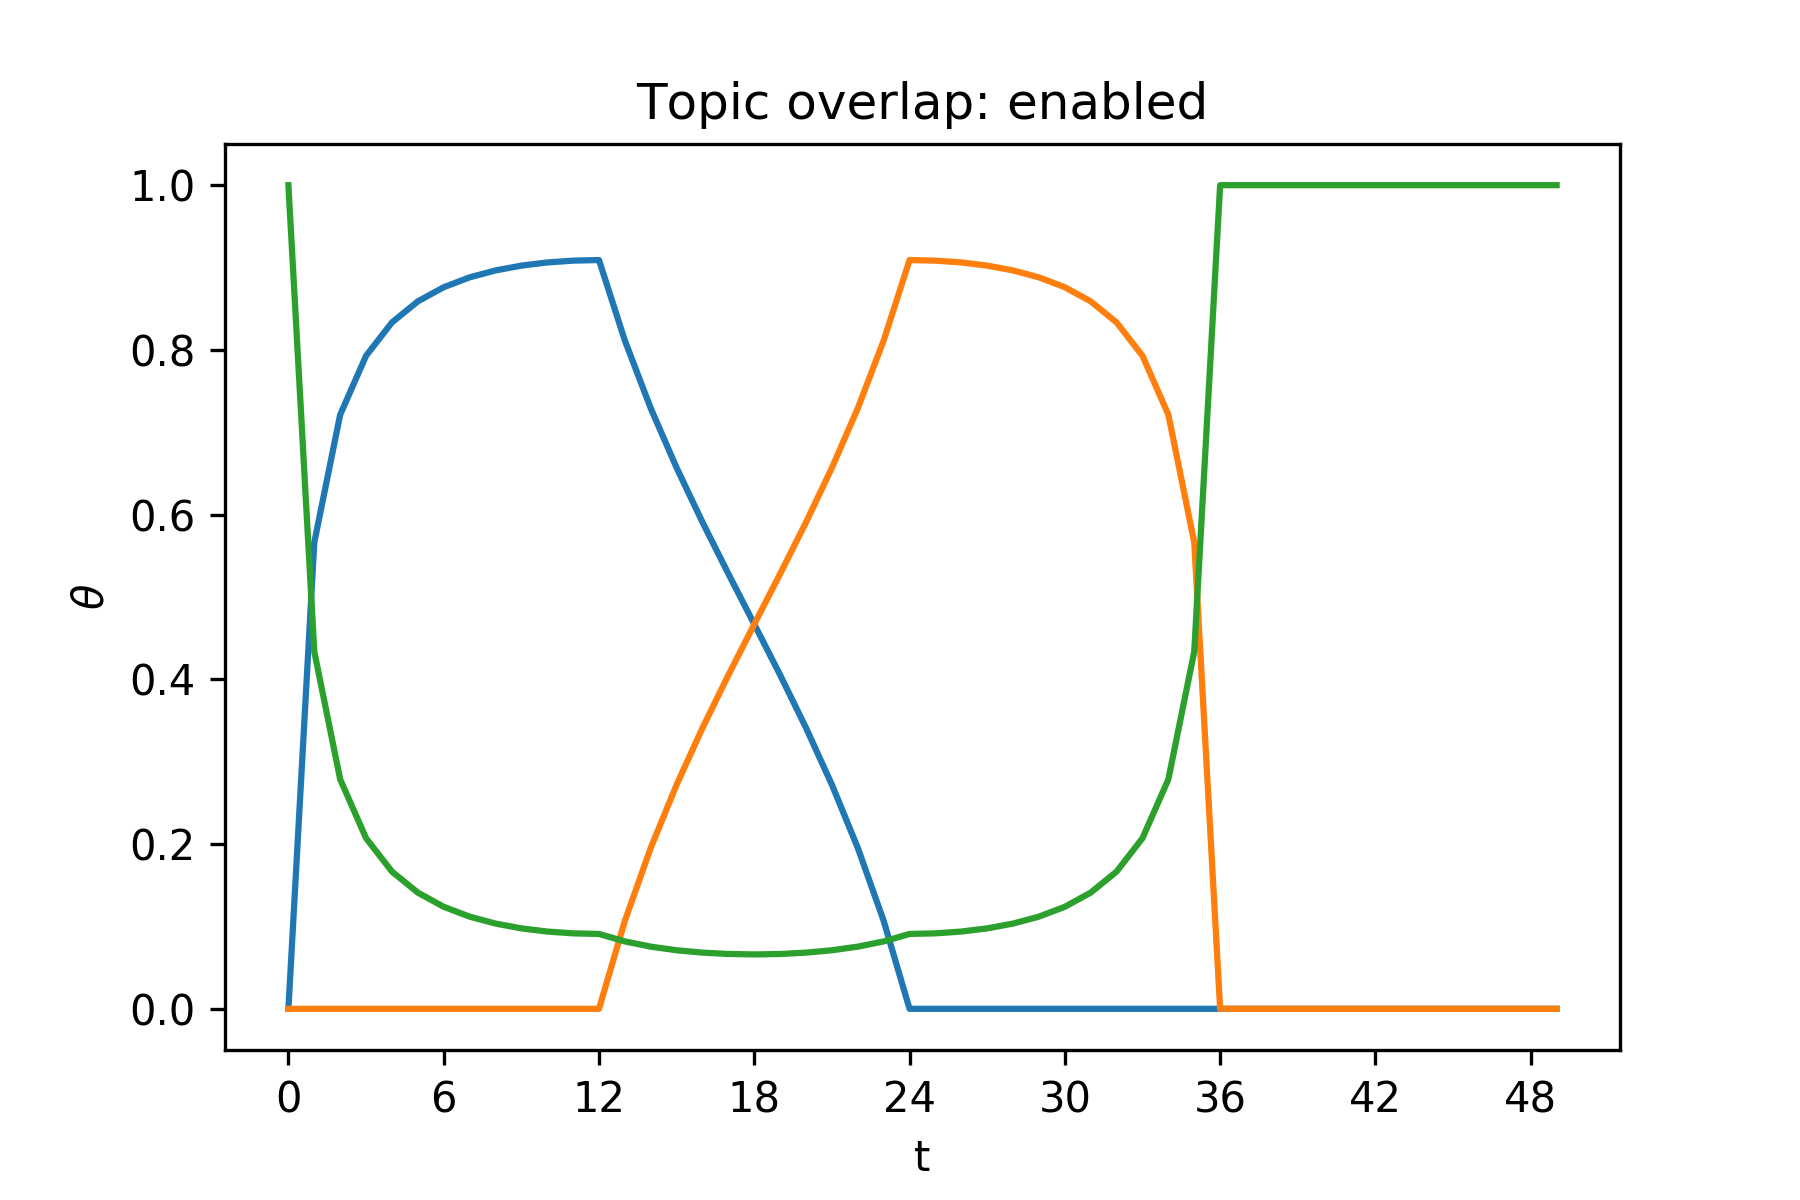
\includegraphics[width=\linewidth]{theta_topic-ol.png}
  \end{subfigure}%

  \begin{subfigure}[b]{0.48\textwidth}
    % \caption{Disabled topic overlap.}
    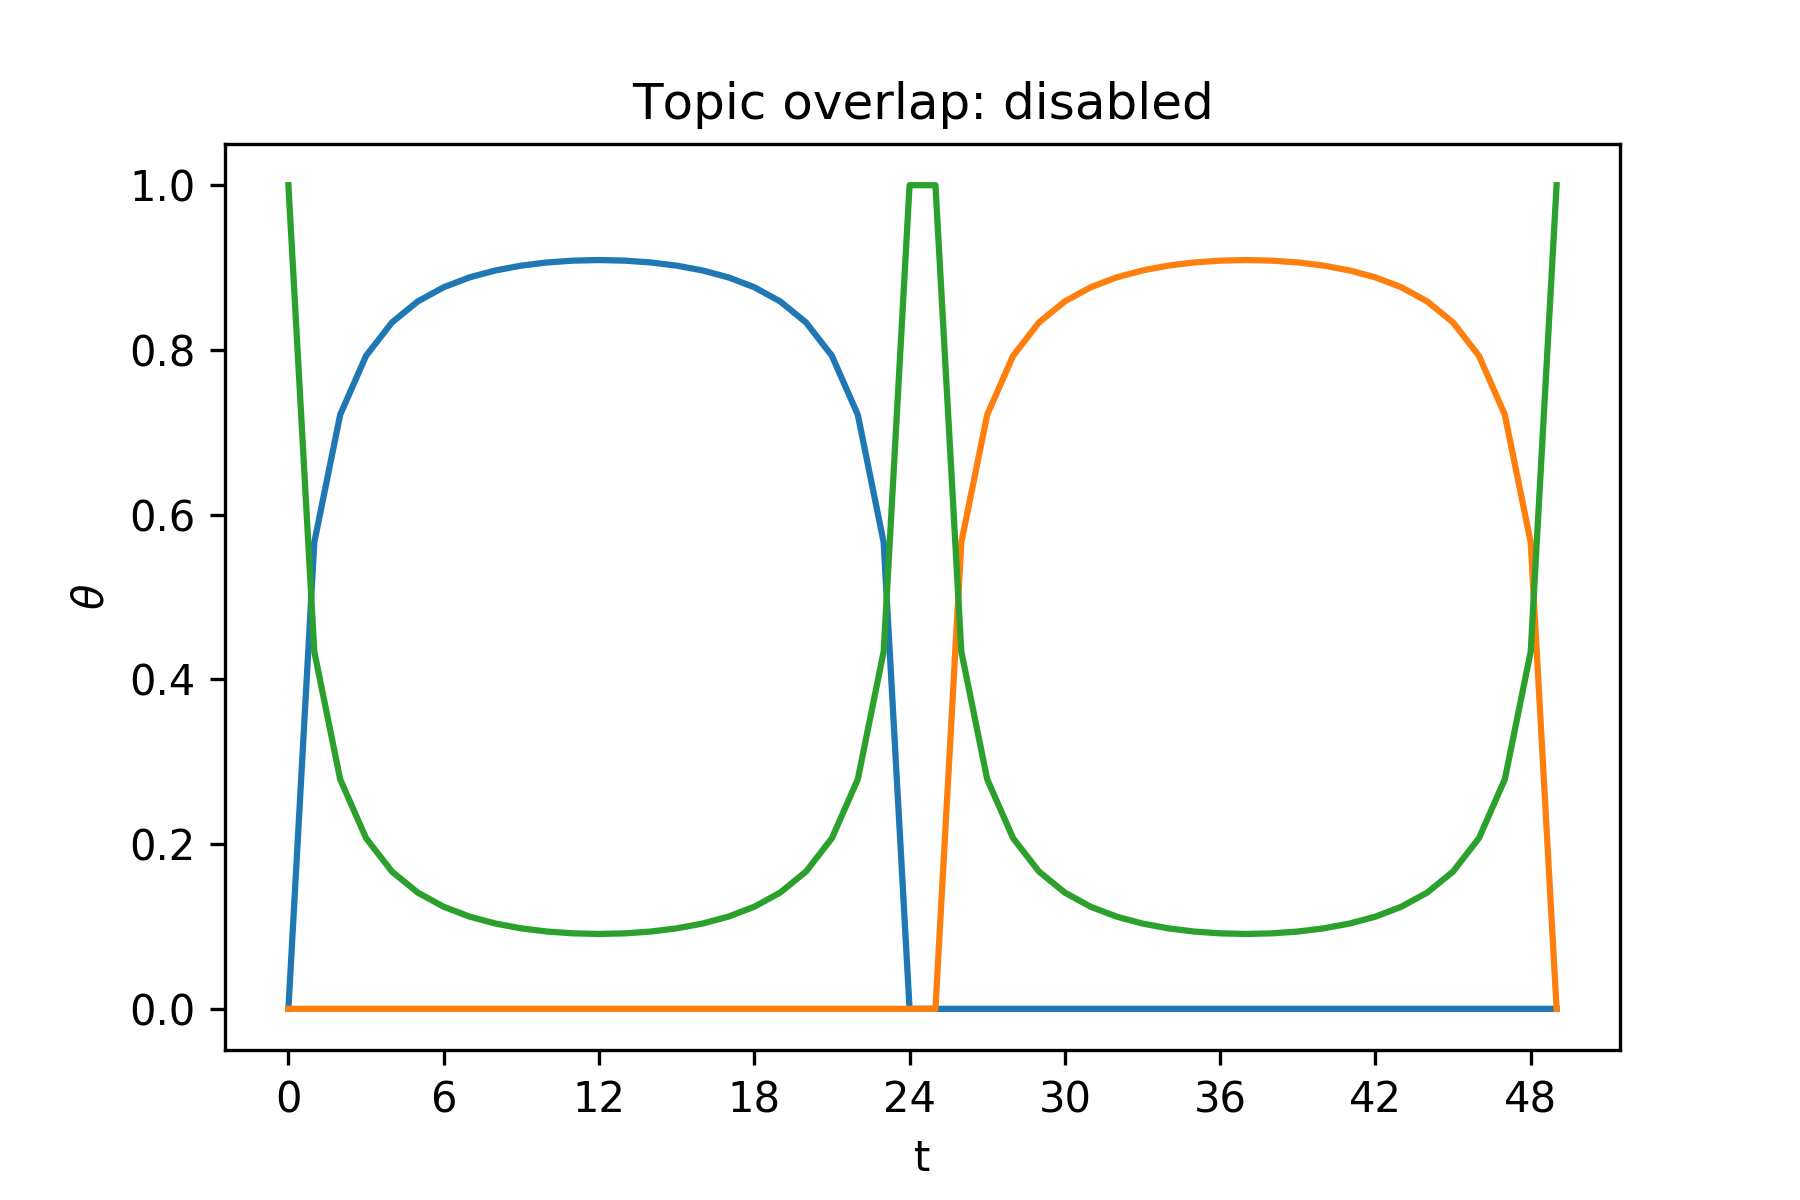
\includegraphics[width=\linewidth]{theta_topic-nonol.png}
  \end{subfigure}%
  \caption{Controlling the topic overlap.}
  \label{fig:ol_topics}

  \begin{subfigure}[b]{0.48\textwidth}
    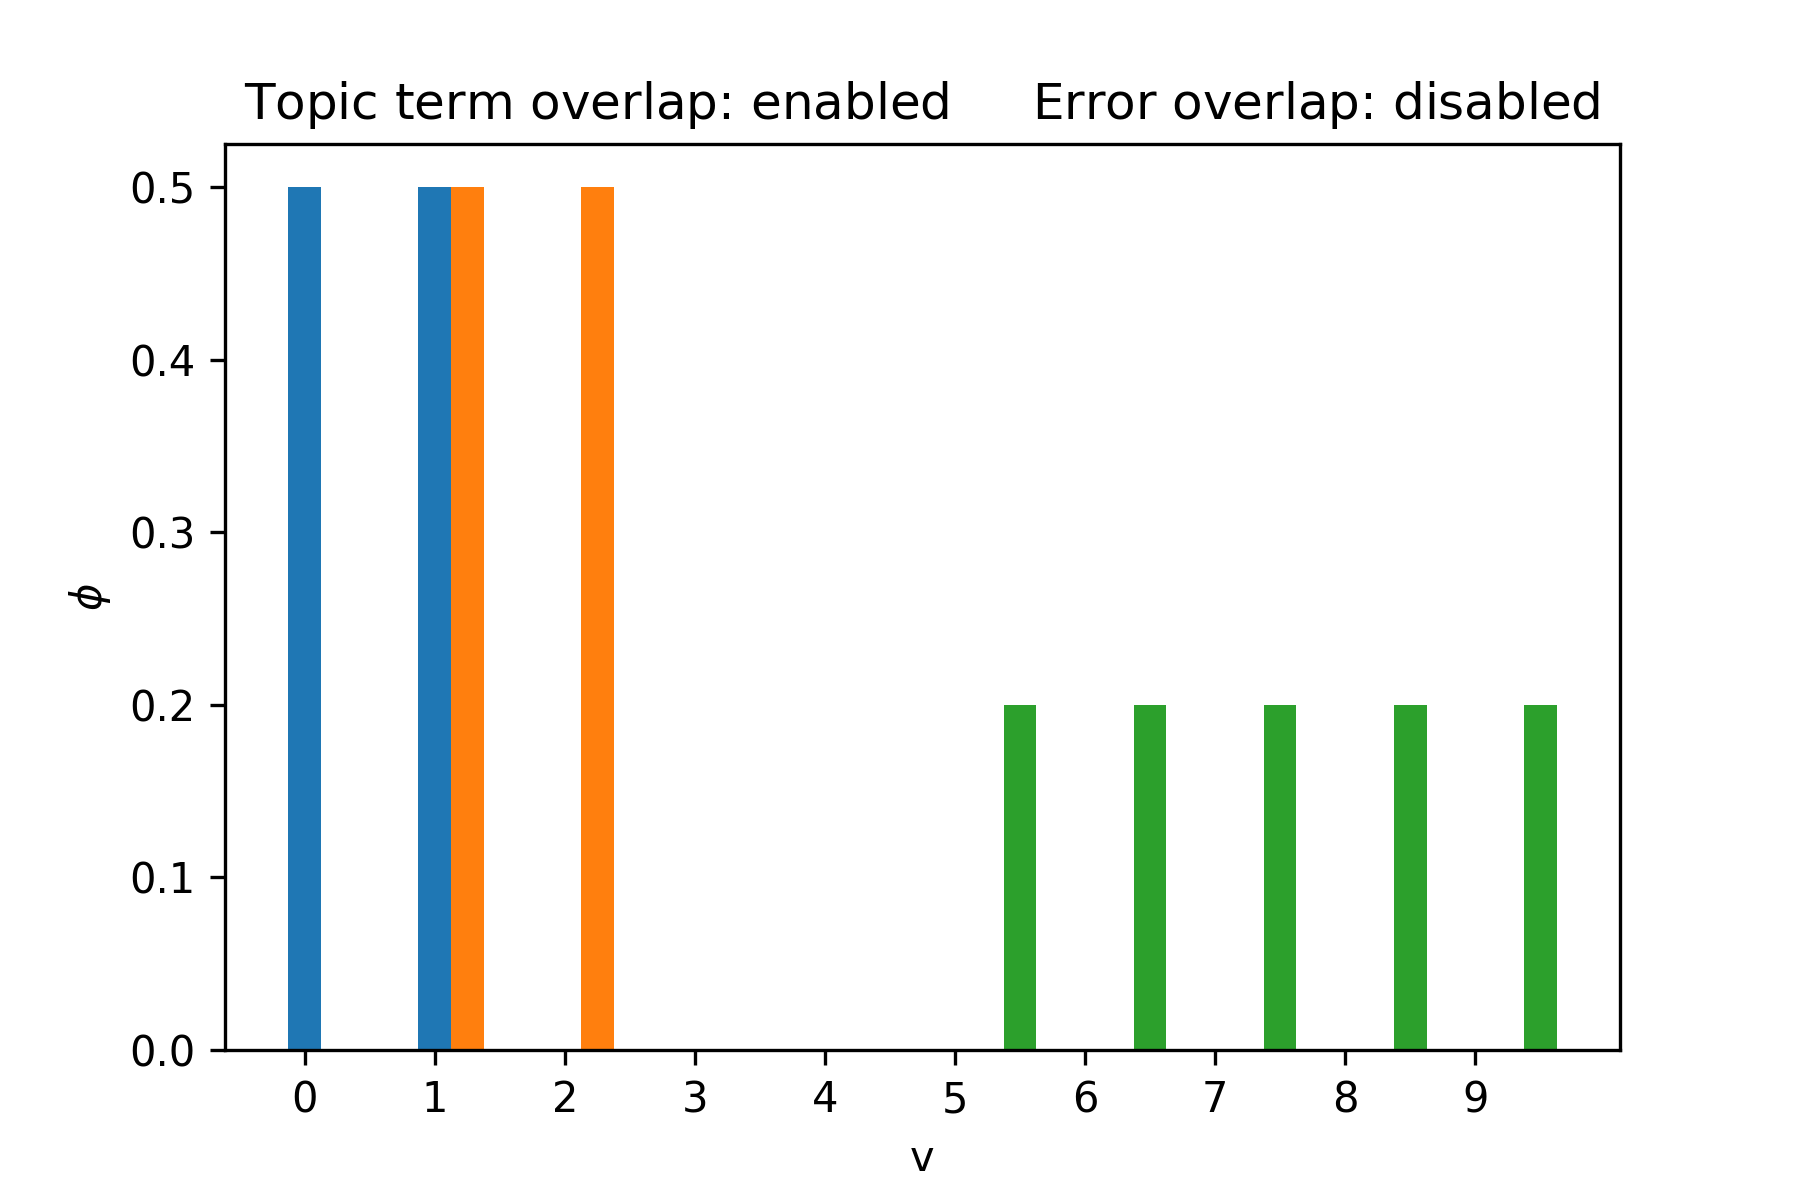
\includegraphics[width=\linewidth]{phi_topic-ol_error-nonol.png}
  \end{subfigure}%
   \caption{Controlling the topic term overlap.}
  \label{fig:ol_terms}

  \begin{subfigure}[b]{0.48\textwidth}
    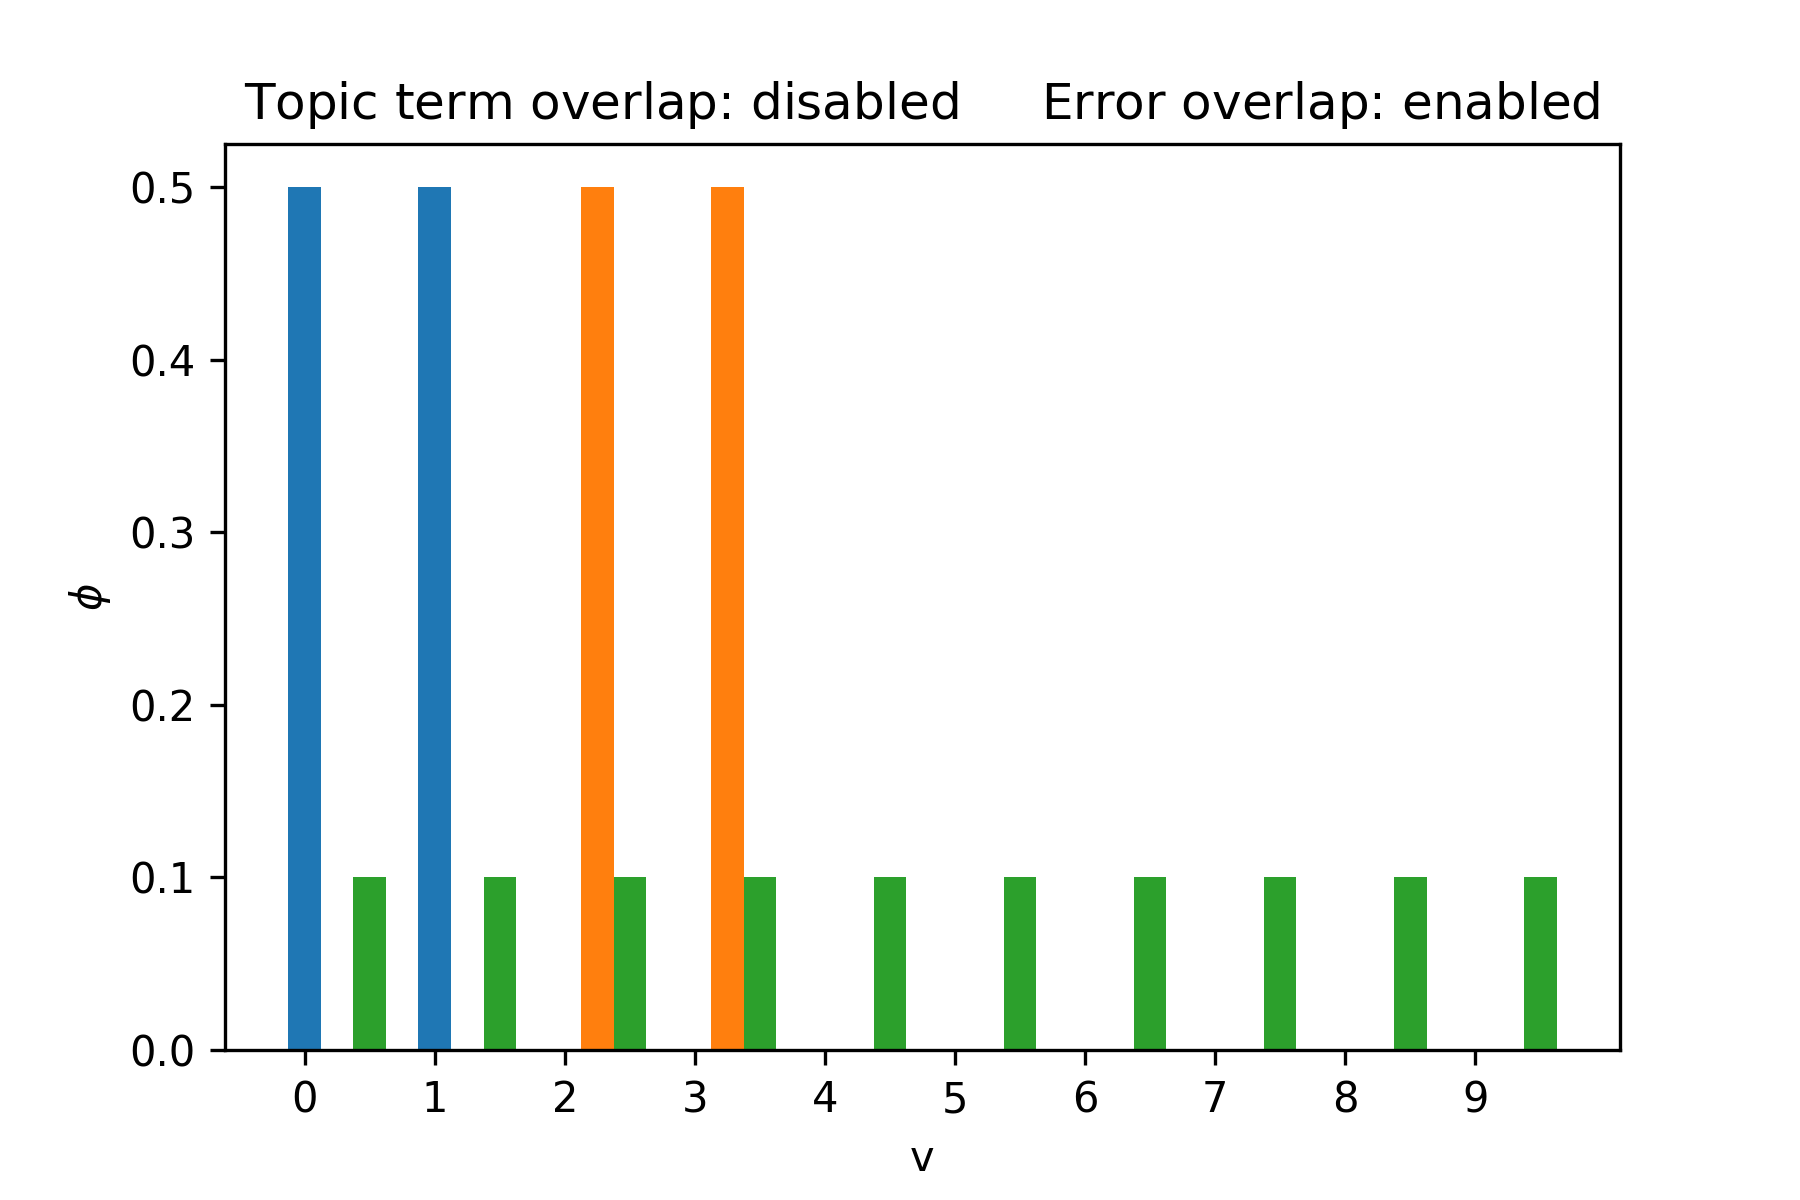
\includegraphics[width=\linewidth]{phi_topic-nonol_error-ol.png}
  \end{subfigure}%
   \caption{Controlling the error overlap.}
  \label{fig:ol_error}
\end{figure}

% Topic model settings
% - AR Tuning
\par In order to run the experiments in an efficient manner, we identify optimal values of the previously noted variances. One reason behind the variance tuning corresponds to the rate of convergence upon the application of the MH algorithm. Based on the algorithm's rationale -- a low acceptance rate indicates a slow and stable convergence, whereas a high acceptance rate indicates a random and unstable convergence -- we would find the variance $\delta^2$ inducing the acceptance rate of around $30\%$. Another reason behind the variance tuning is related to the spatial smoothing application. Most importantly, we keep the variance $\sigma^2$ in tact with the rate of change of the topic smoothing throughout the data. Furthermore, since the topic development is captured in discrete space, we want to make sure that the discretisation step induced by the generative data process is smaller than the $\sigma^2$ variance; otherwise, we would fail to capture the high rate of change induced by steep topic changes.
% MSI data settings
% - Synthetic corpora
% -- Fixed theta and phi
% -- The size of the synthetic corpus 
\par To comment on the datasets generated for the experiments, these are designed to reflect the three following aspects: the effect of overlapping topics; the effect of overlapping vocabulary terms; and the effect of noise. Note that our assessment is based on an intuitive $3$ topic scenario: $2$ topics model distinct metabolite entities, and the remaining topic models the noise topic. To comment on the dataset size, we set $T=50$ for the number of documents per corpus and $\xi=100$ for the number of words per documents: the choice of $T$ surpasses the discretisation concern; also, as suggested by the generative algorithm given in Subsection 5.3, the use of the $\xi$ parameter establishes a slightly varying number of words in each document. However, in order to speed up the inference, we normalise the number of words per document to possess the maximum value of $50$.

% Experiment settings
% - Overlapping topics
% - Overlapping vocabulary terms
% - Overlapping noise vocabulary terms
\par In the following figures, we illustrate the variations of the data generation settings: in Figure \ref{fig:ol_topics}, we display the setting  controlling the topic overlap; in Figure \ref{fig:ol_terms}, we display the setting controlling the topic term overlap; and in Figure \ref{fig:ol_error}, we display the setting controlling the error overlap. Note that the red and green colourings indicate the synthetic metabolite topics; the green colouring indicates the noise topic; and, for the term names set in the horizontal axes of Figures \ref{fig:ol_terms} and \ref{fig:ol_error}, we use arbitrary, unique numbers. 

% Experiment settings
% - Illustration overview: example
% - preset theta and phi
\par Relating the latter settings to our experiments, we assess their all (eight) possible permutations. To give an example of a permutation, one of the experiments would assess the ability to recover the underlying topic term distributions with the enabled topic overlap, the disabled topic term overlap, and the enabled error overlap. Note that the latter settings directly reflect the $\theta$ and $\phi$ values of the synthetic datasets (we do not use the $\alpha$ and $\beta$ hyper-parameters). By following the latter principle, we establish a clearer representation of the synthetic data; thus, simplify the performance assessment.

\subsection{Experiment execution}

% Evaluation
% - Performance: topic and term recreation error

\par Before going into the experiment execution, note that we assess the performance based on the models' ability to recover the underlying synthetic corpus generation settings. To wrap this assessment into a more concise terminology, the true solution corresponds to the underlying synthetic corpus generation settings; and the approximate solution corresponds to the inference results. As a result, the performance is measured by taking the difference between the true and approximate solutions. 

% Specific examples
% - # of iter & burn-in
\par In order to introduce the rationale behind the performance assessment, we look into one of the eight experiments in more detail. Just like for all our experiments, we run both auto-regressive and non-auto-regressive models for $5000$ Gibbs sampling iterations, $1000$ of which are dedicated to the burn-in process. For each of the remaining $4000$ iterations, we sample the corresponding $\theta$ and $\phi$ values; afterwards, in every $100$th iteration, we average the stored $\theta$ and $\phi$ values, respectively; then, this average is compared to the true solution. As an example, in the $1100$th iteration, we would take the average of $100$ samples; in the $1200$th iteration, we would take the average of $200$ samples. In a single experiment, we would have $40$ of such batches indicating the performance -- this is illustrated in Figure \ref{fig:perf_theta} and Figure \ref{fig:perf_phi}.

\begin{figure}[h]
  \centering
  \begin{subfigure}[b]{0.37\textwidth}
    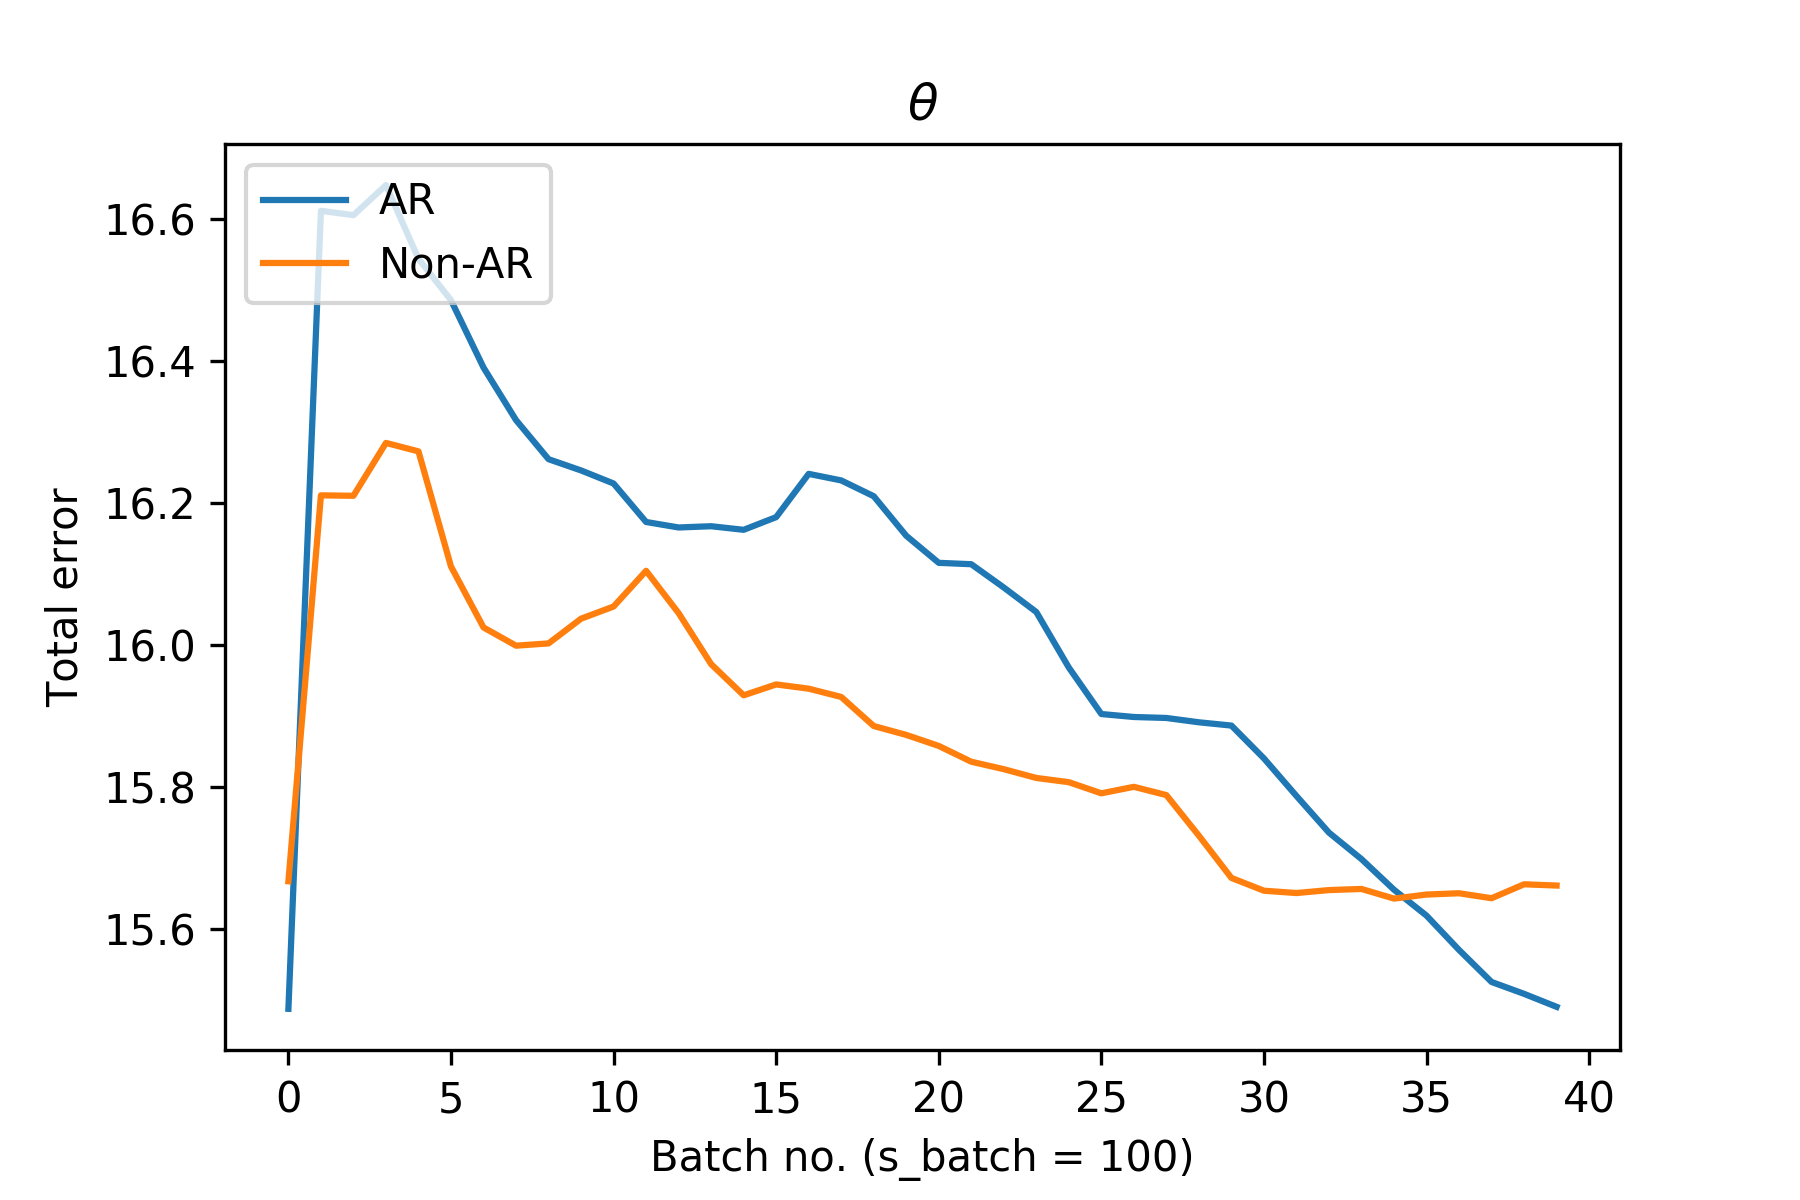
\includegraphics[width=\linewidth]{performance-theta.png}
  \end{subfigure}%
  \caption{The $\theta$ recovery performance.}
  \label{fig:perf_theta}
  \begin{subfigure}[b]{0.37\textwidth}
    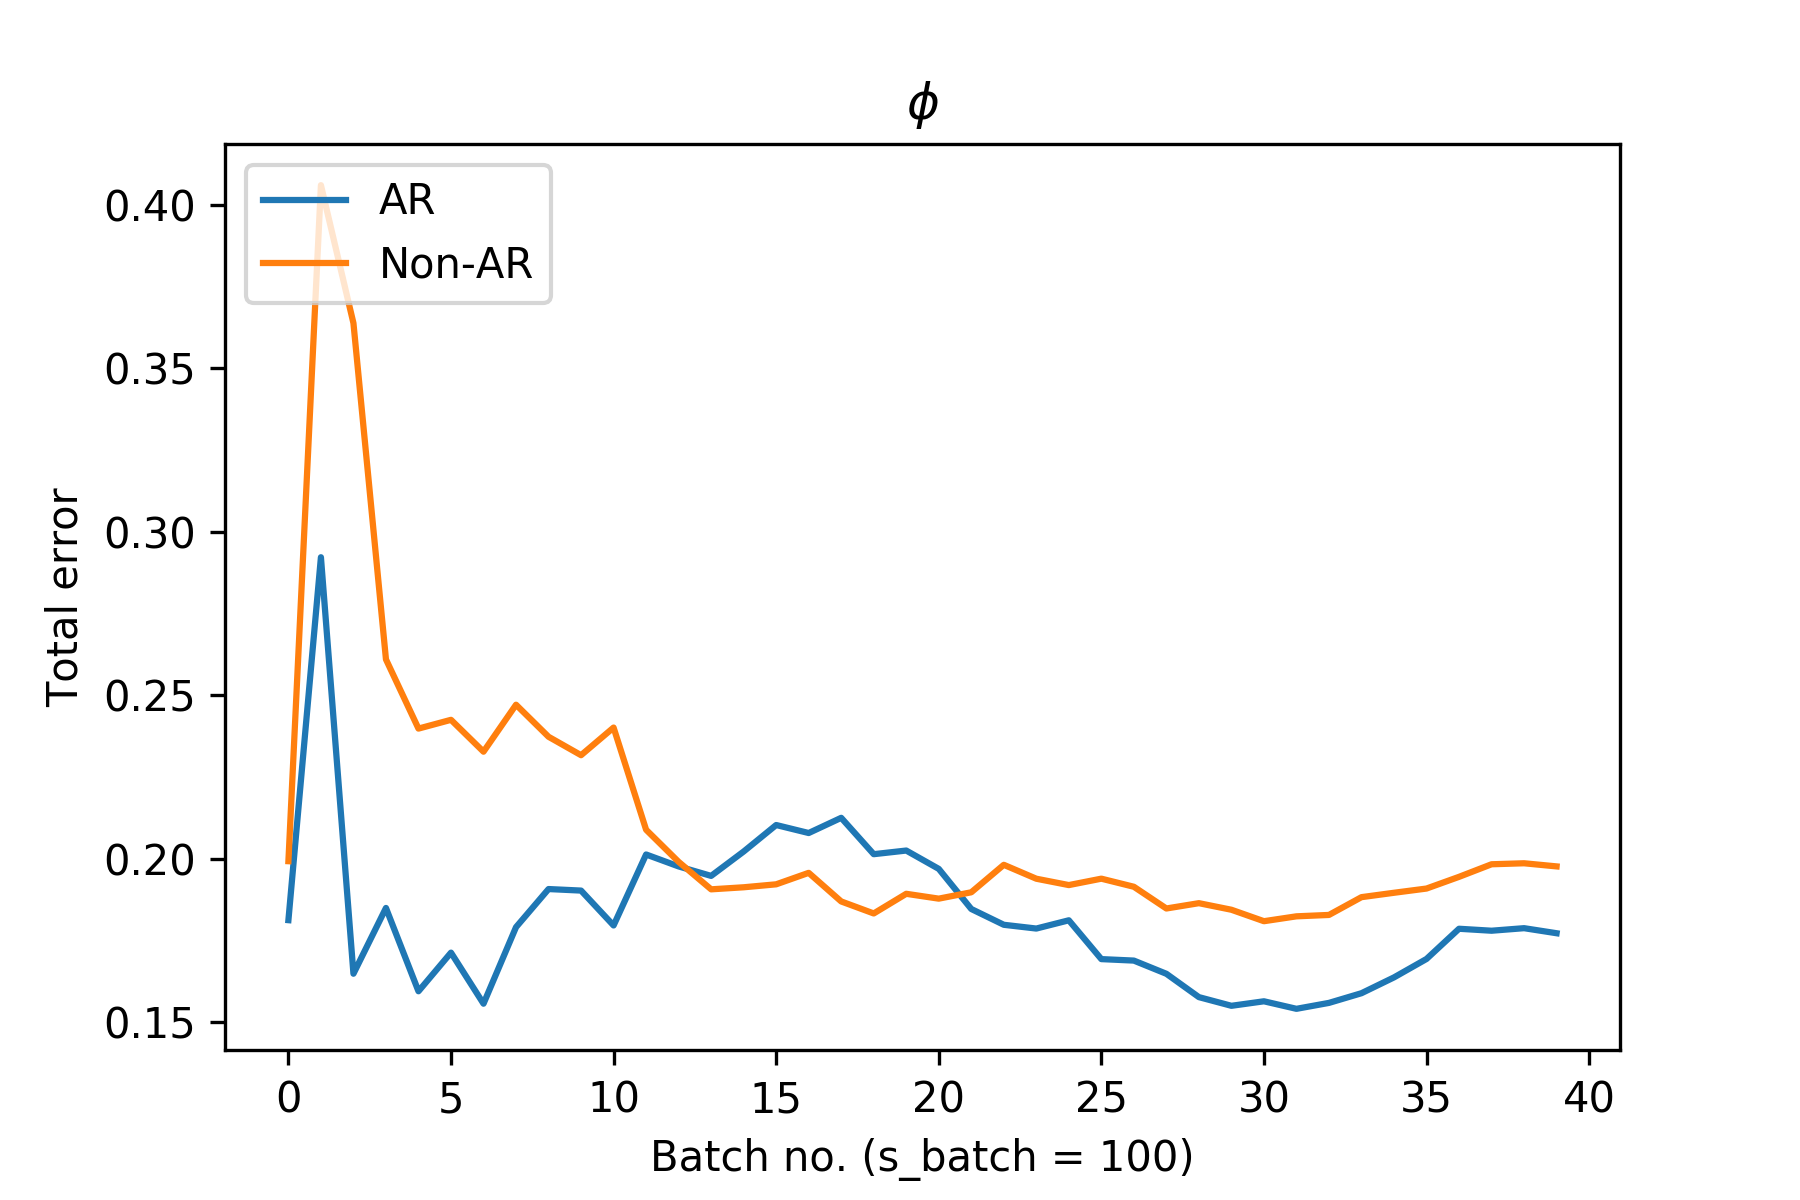
\includegraphics[width=\linewidth]{performance-phi.png}
  \end{subfigure}%
  \caption{The $\phi$ recovery performance.}
  \label{fig:perf_phi}
\end{figure}

% The images of theta and phi recovery
\par Relating to the previous example, the $\theta$ and $\phi$ values corresponding to the last iteration are illustrated in Figure \ref{fig:comp_theta} and Figure \ref{fig:comp_phi}, respectively. Also, note that we relax the colour coding of our figures as the topics are inferred in unsupervised manner.

\begin{figure}
  \centering
  \begin{subfigure}[b]{0.48\textwidth}
    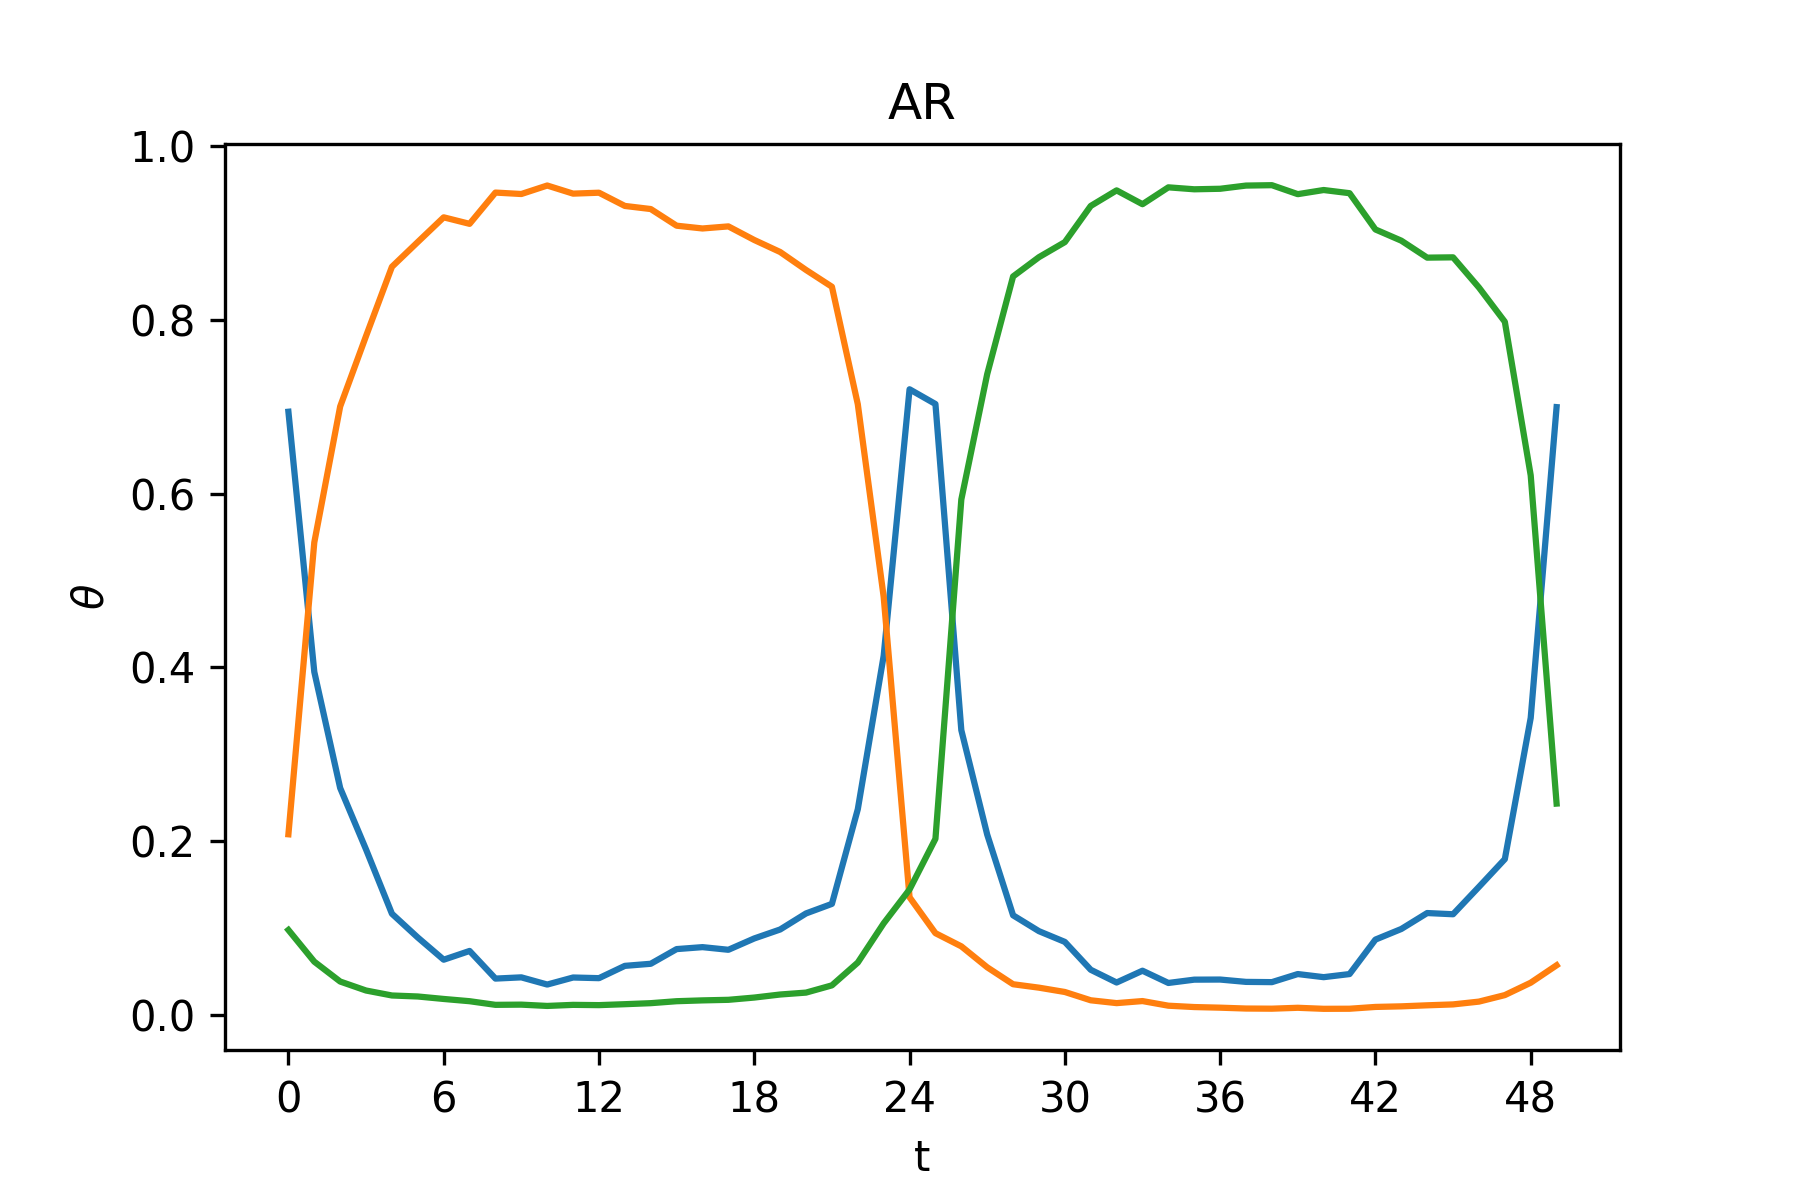
\includegraphics[width=\linewidth]{theta-ar_11.png}
  \end{subfigure}%

  \begin{subfigure}[b]{0.48\textwidth}
    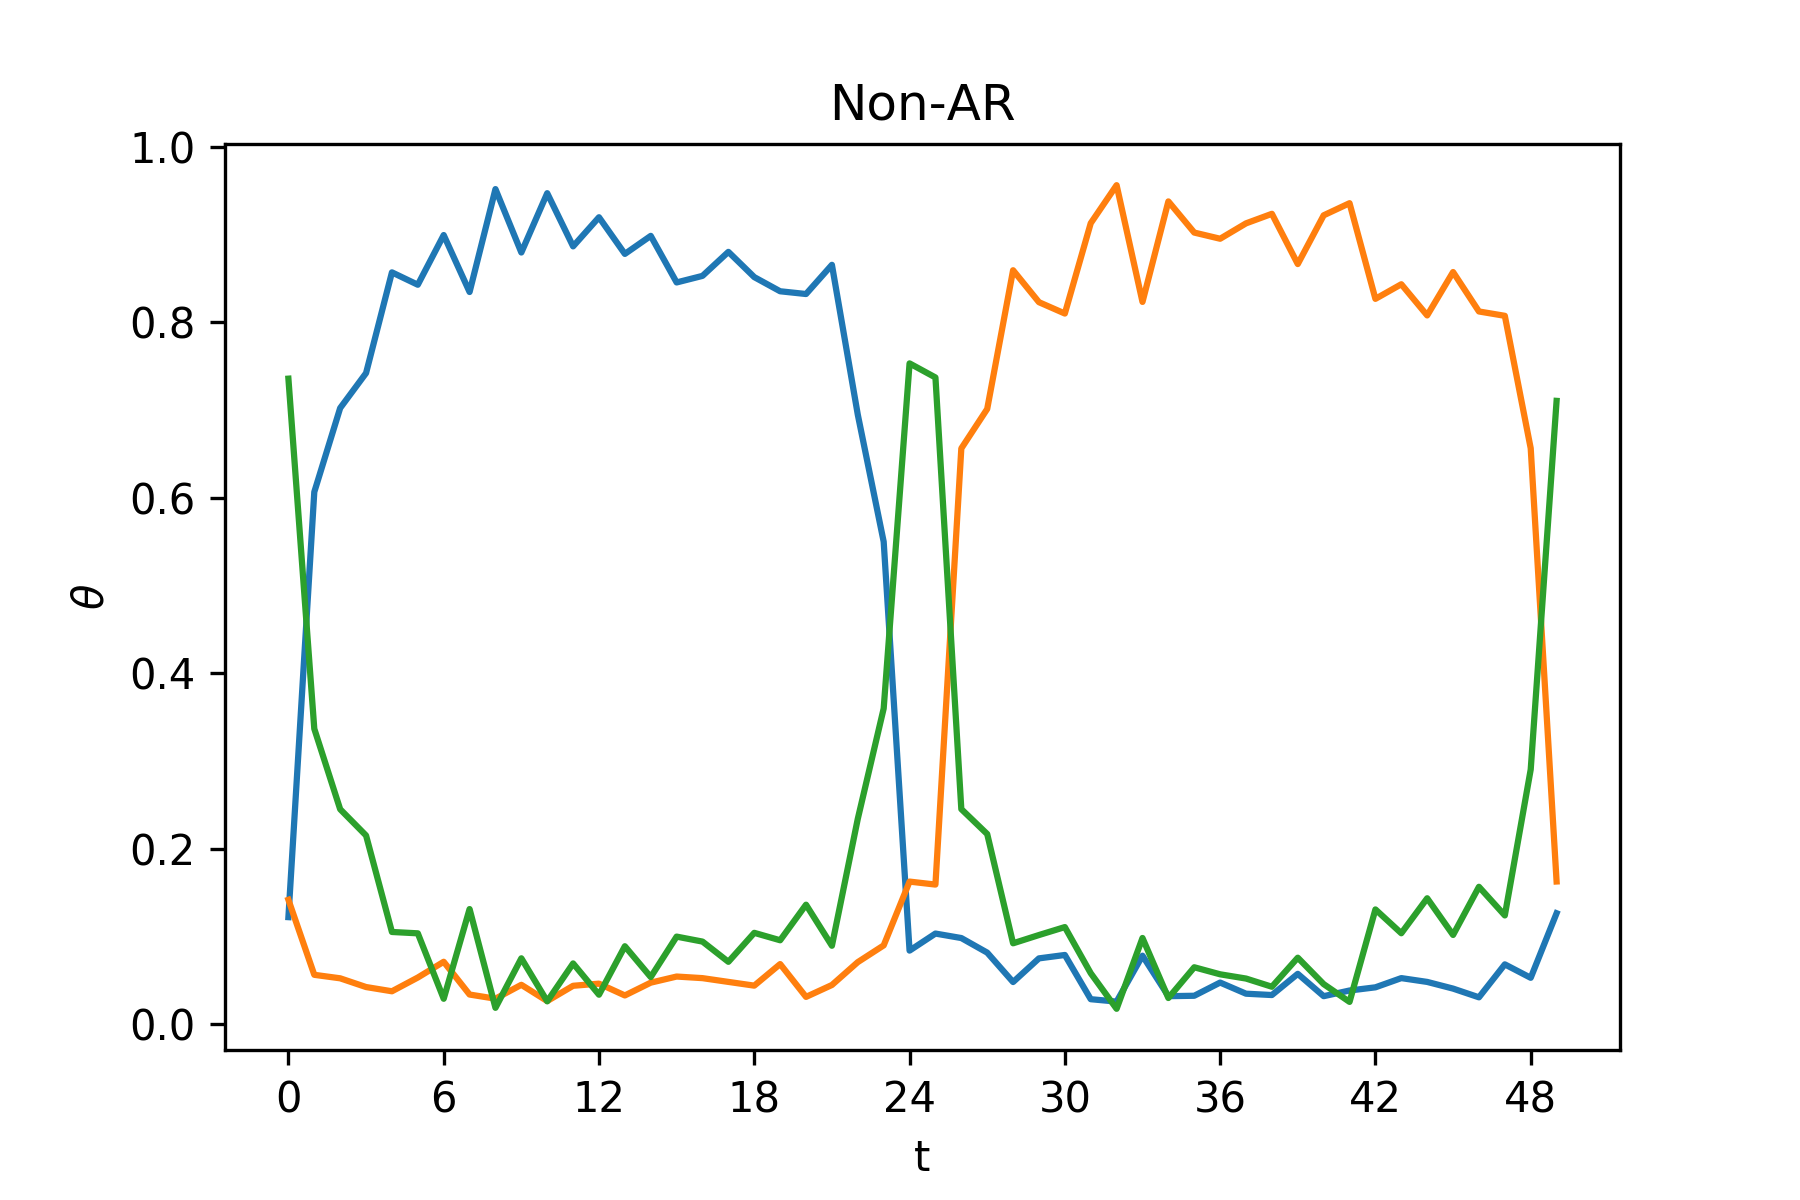
\includegraphics[width=\linewidth]{theta-nonar_11.png}
  \end{subfigure}%
  \caption{The comparison of the $\theta$ values.}
  \label{fig:comp_theta}

  \begin{subfigure}[b]{0.48\textwidth}
    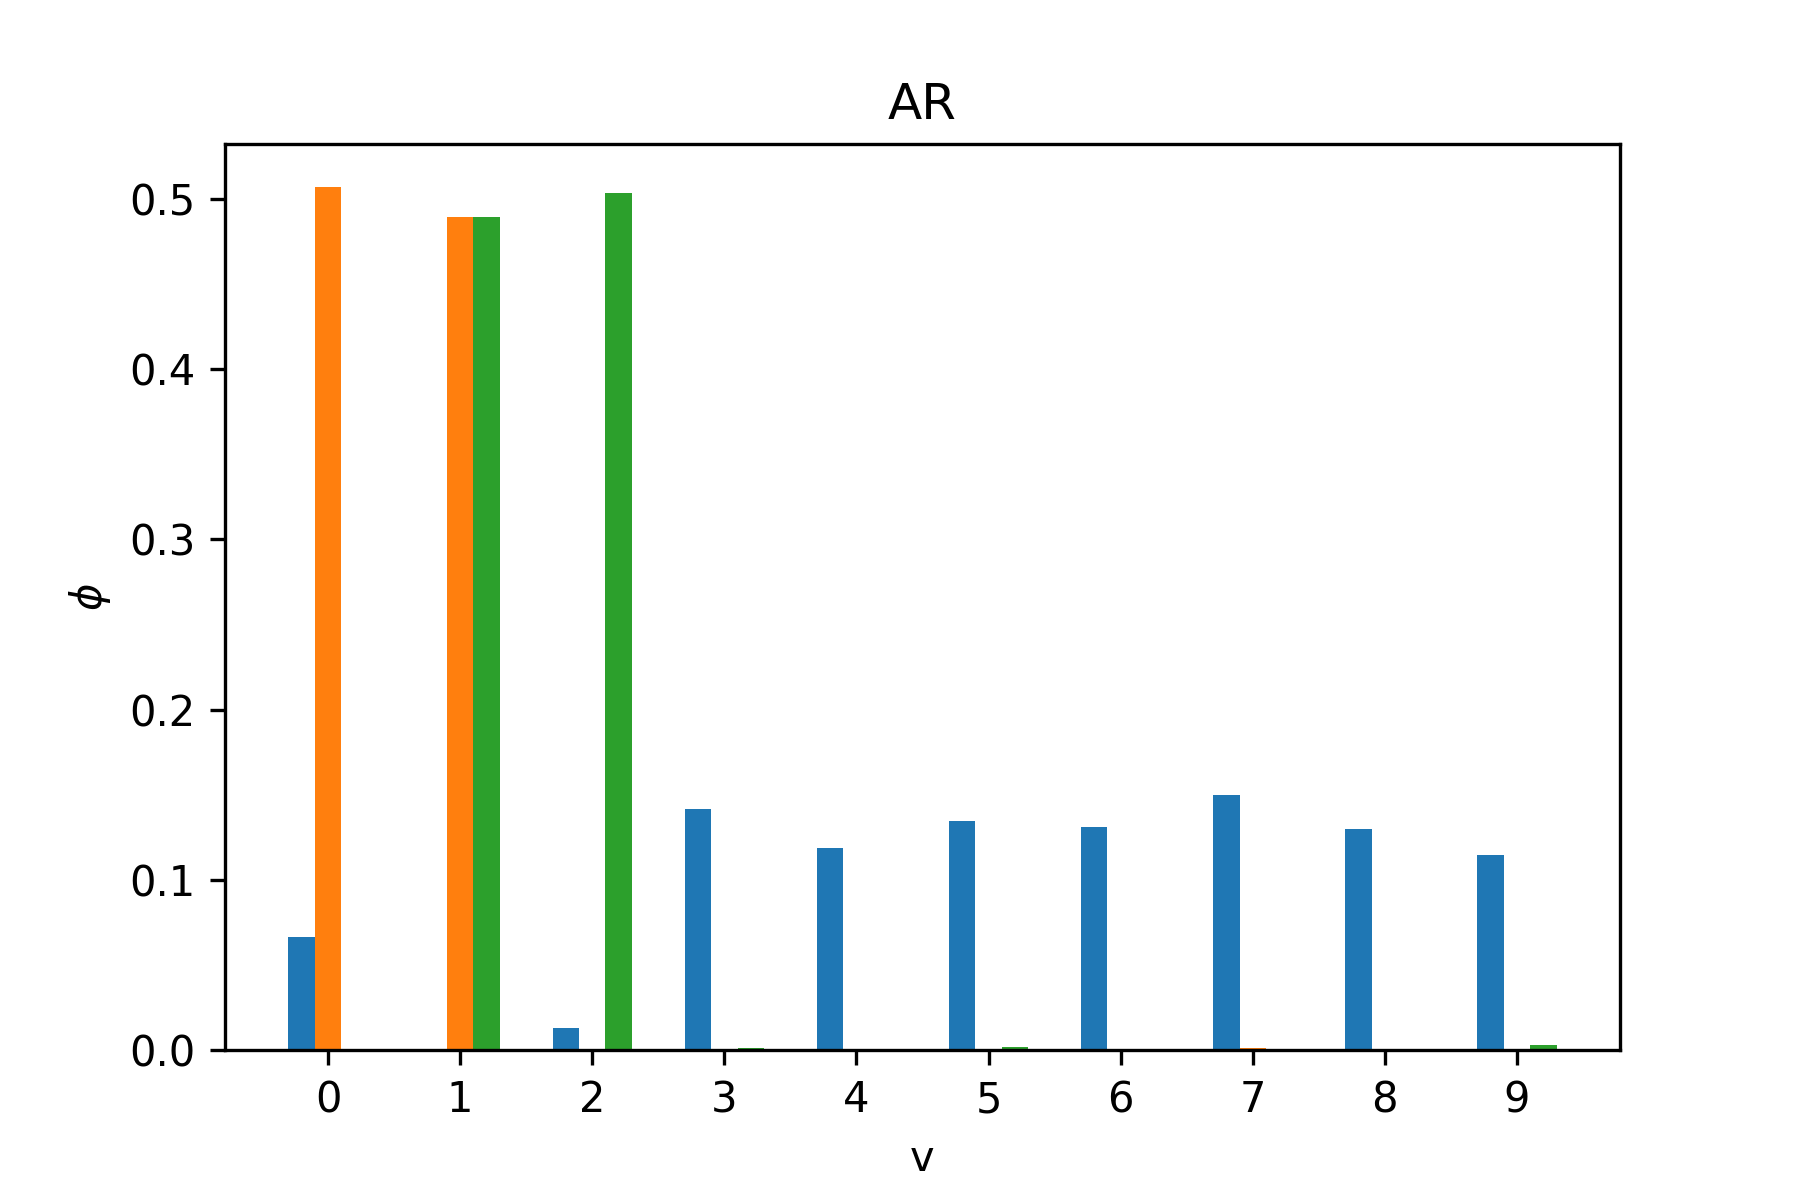
\includegraphics[width=\linewidth]{phi-ar_11.png}
  \end{subfigure}%

  \begin{subfigure}[b]{0.48\textwidth}
    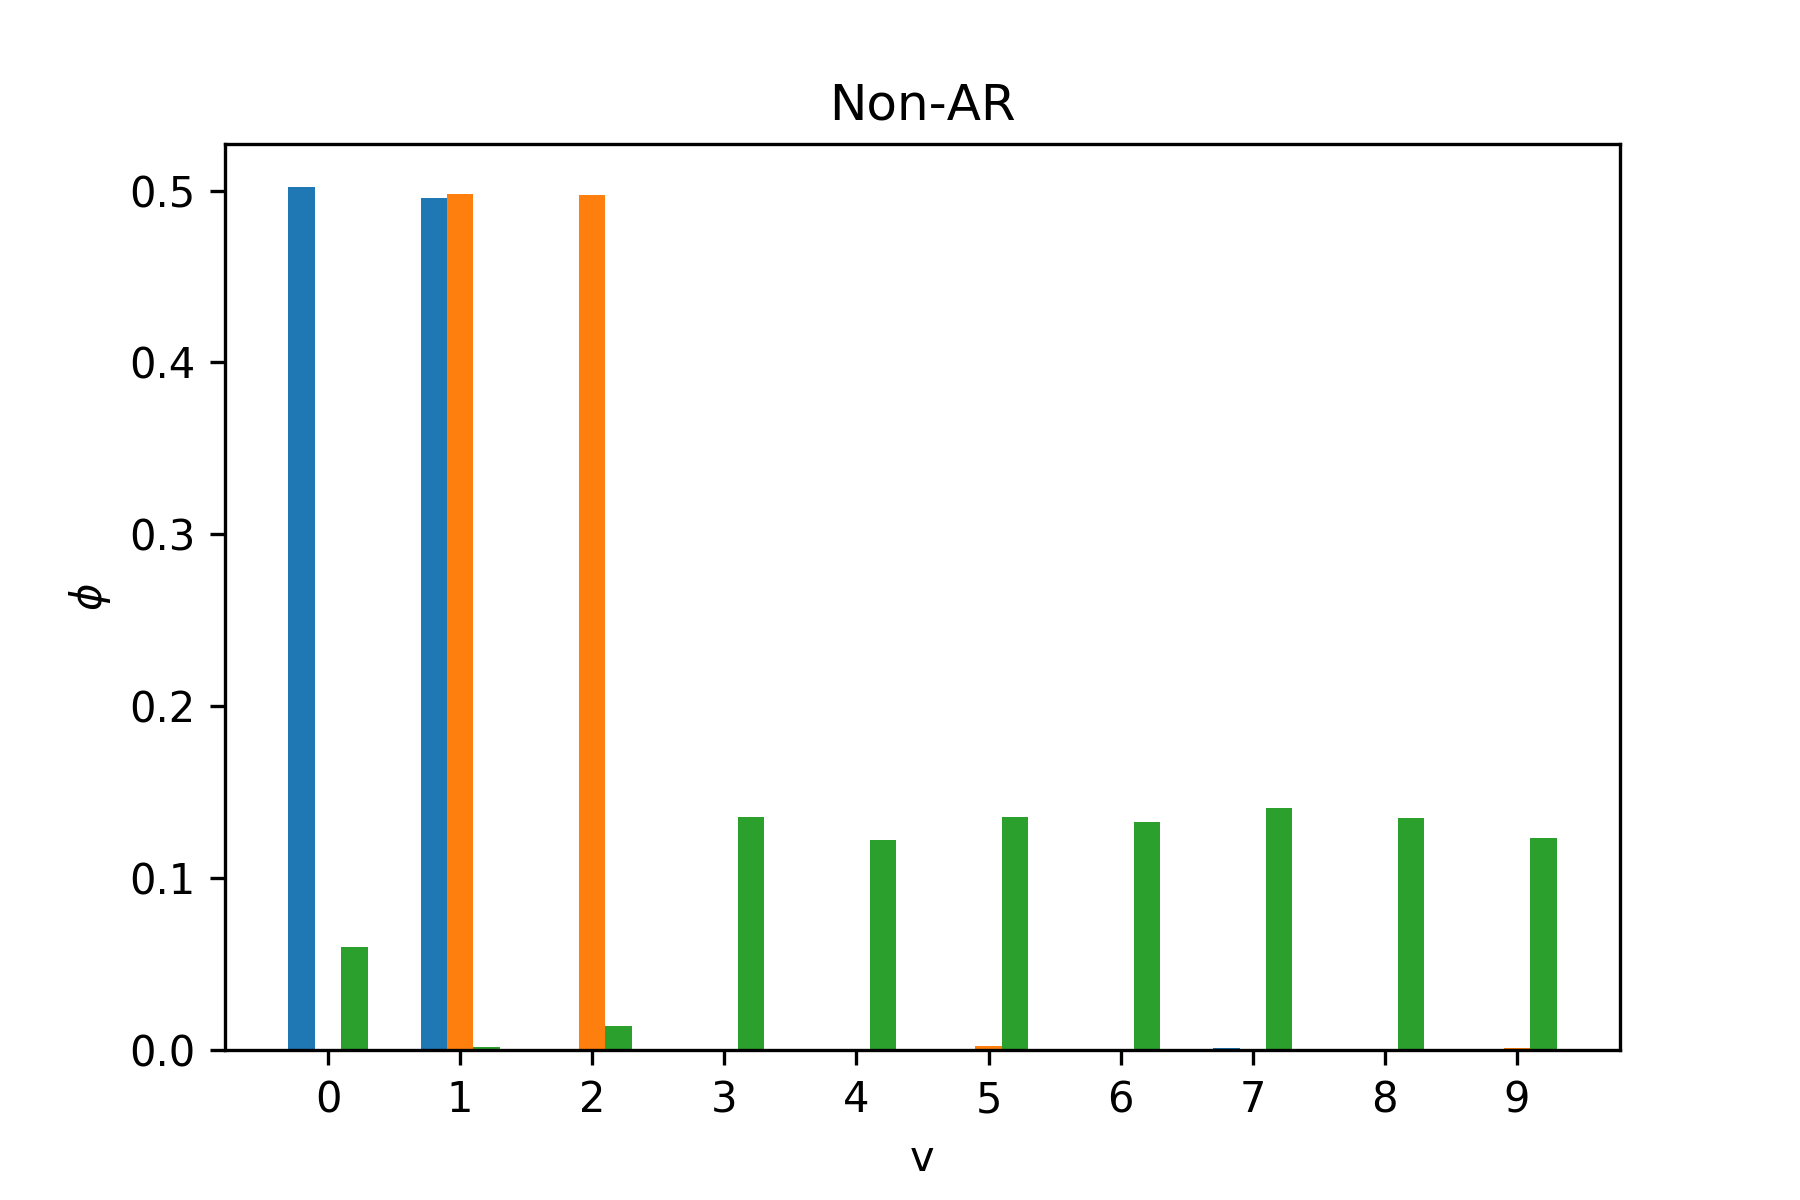
\includegraphics[width=\linewidth]{phi-nonar_11.png}
  \end{subfigure}%
  \caption{The comparison of the $\phi$ values.}
  \label{fig:comp_phi}
\end{figure}
 
% General assessment
% - The table with the paired t-test scores
% - Paired t-test
% -- 10 datasets each
\par To assess the auto-regressive model's performance, we have generated $10$ distinct datasets for each previously introduced corpus generation setting. Recall that we assess the following conditions: the topic overlap; the vocabulary term overlap; and the error term overlap. For every setting permutation, we perform the two-tailed t-test: the t-statistic suggests the difference in performance; and the p-value suggests whether the result is significant. To be more specific, a negative t-statistic indicates the auto-regressive model's superior performance; whereas the results are determined to be significant if the p-value is below $0.05$. The t-statistics and p-values of all eight performed experiments are provided in Table \ref{tab:ttest} below.

\begin{table}[H]
\begin{center}
\begin{tabular}{|>{\centering\arraybackslash}p{0.75cm}|>{\centering\arraybackslash}p{0.75cm}|>{\centering\arraybackslash}p{0.75cm}">{\centering\arraybackslash}p{0.75cm}|>{\centering\arraybackslash}p{0.75cm}|>{\centering\arraybackslash}p{0.75cm}|>{\centering\arraybackslash}p{0.75cm}|} 
\hline
\multicolumn{3}{|c"}{Overlap} &
\multicolumn{2}{c|}{t-statistic} &
\multicolumn{2}{c|}{p-value} \\
\hline
% \hline
Topic & Term & Error & $\theta$ & $\phi$ & $\theta$ & $\phi$ \\
\thickhline
False & True & True & $-5.41$ & $0.47$ & $0.00$ & $0.65$ \\
False & True & False & $-9.46$ & $-0.38$ & $0.00$ & $0.71$ \\
False & False & True & $4.74$ & $3.93$ & $0.00$ & $0.00$ \\
False & False & False & $-2.91$ & $-3.24$ & $0.02$ & $0.01$ \\
True & True & True & $-5.99$ & $-1.71$ & $0.00$ & $0.12$ \\
True & True & False & $-1.78$ & $-1.53$ & $0.11$ & $0.16$ \\
True & False & True & $1.12$ & $1.17$ & $0.29$ & $0.27$ \\
True & False & False & $0.52$ & $1.10$ & $0.61$ & $0.30$ \\
\hline
\end{tabular}
\end{center}
  \caption{The t-test assessing 8 different overlap settings.}
  \label{tab:ttest}
\end{table}

% - Commenting on the significant results
\par Based on the obtained results, the most significant changes (the p-values vary from $0.00$ to $0.01$) occur upon only switching the error overlap setting (the remaining settings are disabled). If the error overlap is disabled, the spatial smoothing application displays an improved performance (i.e., $3.24$ lower error in recovering $\phi$); however, if the setting is enabled, the auto-regressive model performs poorly (i.e., $3.93$ higher error in recovering $\phi$). Further, by relaxing the significance threshold, we can also consider the experiment instances where the p-values vary from $0.12$ to $0.16$. Conveniently, in this experiment pair, we again consider only the switch of the error overlap setting; however, in this case, all other settings are enabled. To comment on the respective performance, the spatial smoothing application is superior in both cases: $1.71$ and $1.53$ lower error rates in recovering $\phi$.

% - Result pairing
% - Notes why some results are insignificant
\par Interestingly, we can group the experiment listings in four pairs: the pairs are centred around the $\phi$ p-values of $0.01$, $0.16$, $0.30$, or $0.71$. The first two pairs are presented in the previous paragraph; however, for the last two pairs, the p-values are well beyond the significance threshold. By noting that, in every pair, only the error setting varies, the insignificant results occur when one of the topic and term settings is disabled and another is enabled. By looking into the $\phi$ recovery plots related to the insignificant results, we noticed that both auto-regressive and non-auto-regressive models infer similar latent $\phi$ distributions. Effectively, in the case of the enabled error setting, both models simplify the dataset complexity; that is, the models assign the overlapping error terms to the main topics. Alternatively, in the case when the error setting is disabled, the problem is too simple -- both models recover the $\phi$ values equally well. To give an example of a similar performance, the reader can consider the previously introduced Figure \ref{fig:perf_phi} and Figure \ref{fig:comp_phi}. However, by examining Figure \ref{fig:perf_phi}, note that the $\phi$ value of the auto-regressive model converges faster.

% ___________________________________________________________________________
\section{Conclusion}

% Summary
\par In this research paper, we reviewed an attempt to induce spatial smoothing in MSI data: the research problematic was supported and inspired by covering the relevant literature; the model's design was introduced by providing the preliminary knowledge covering LDA, spatial smoothing, and MSI data pre-processing; finally, the experiment settings were designed to identify both superior and inferior spatial smoothing application prospects.

% Results
% - Comment on the ability to recover phis
\par Our main objectives were to identify the spatial smoothing application's prospect in recovering the $\phi$ values used upon the generative data process and the ability to separate the noise topic. We report that only a half of the carried experiments displayed a significant performance in recovering the $\phi$ values. To be more specific, we observe an improved $\phi$ recovery when the synthetic datasets are generated using enabled topic and terms overlap settings; alternatively, when both topic and term overlap settings are disabled, the performance is superior if the error overlap is disabled and inferior if the error overlap is enabled.

% Results
% - Comments on the ability to find the noise
\par To expand on the overlapping noise topic's identification (i.e. noise detection), the auto-regressive model -- just like the non-auto-regressive model -- assigns the overlapping error terms to the main topics. For this reason, we conclude that the spatial smoothing application is negligible in improving the overlapping noise topic term detection. However, looking into the statistical test on the $\theta$ values, $6$ out $8$ experiments display a significant performance in recovering the $\theta$ values. In $5$ out $6$ cases, the $\theta$ values are recovered with a lower error; this result is mostly impacted by the model's ability to reflect the shape of the noise topic with a better accuracy. 

% Results
% - Comment on the further prospects
% -- Spatial smoothing multi-neighbour
\par Since some of the experiment settings display a performance improvement, the spatial smoothing application could be considered for a further research. We would recommend looking into the application of the undirected graphical model -- Markov random field. Effectively, the application would establish more complex spatial smoothing settings: the spatial treatment of neighbouring entities could be improved from 1-dimensional to 2- or 3-dimensional. Effectively, the spatial dimensionality escalation would reflect the visual aspect of MSI data better. 

% Future prospects
% - bucketisation
\par To suggest an alternative research direction in assessing the spatial smoothing application, we propose a research problem on investigating bucketisation enhancements. In other words, the spatial smoothing application might have an impact upon the feature extraction from MSI data. To be more specific, spatial smoothing might establish more appropriate bucket size ranges in concatenating raw mass-to-charge values. If successful, this application would improve the quality of MSI data features and, consequently, improve the performance of the research problems addressed by this research project. 

% - Comment on identifying appropriate settings
% -- All disabled settings do not display a metabolomics-like environment
\par To give the final verdict on the research project's outcome, we consider the performance obtained using the settings reflecting the metabolomics environment the best. Effectively, the more overlap settings are enabled, the better the metabolomics environment is represented. As shown by Table \ref{tab:ttest}, the auto-regressive model tends to perform better when most of the overlap settings are enabled. Therefore, we conclude that spatial smoothing can be indeed effective on improving the assessment of the MSI data with metabolomics environment characteristics.

% ___________________________________________________________________________
\bibliographystyle{abbrv}
\bibliography{bibliography}

\end{document}

	